\documentclass[12pt, a4paper]{article}

% ── Packages ──────────────────────────────────────────────────────────────────
\usepackage[T1]{fontenc}
\usepackage[utf8]{inputenc}
\usepackage[english]{babel}
\usepackage{lmodern}
\usepackage{microtype}

\usepackage{amsmath, amssymb, amsthm}
\usepackage{mathtools}

\usepackage{geometry}
\geometry{top=2.5cm, bottom=2.5cm, left=3cm, right=3cm}

\usepackage{graphicx}
\usepackage{float}
\usepackage{subcaption}
\usepackage{booktabs}
\usepackage{array}

\usepackage{xcolor}
\usepackage{hyperref}
\hypersetup{
    colorlinks=true,
    linkcolor=blue!70!black,
    citecolor=blue!70!black,
    urlcolor=blue!70!black
}

\usepackage{setspace}
\onehalfspacing

\usepackage{parskip}
\setlength{\parindent}{0pt}
\setlength{\parskip}{6pt}

% ── Title ─────────────────────────────────────────────────────────────────────
\title{\textbf{High-Dimensional Macroeconomic Forecasting: A Model Comparison}\\[4pt]
       \large An Exercise Based on De Mol, Giannone \& Reichlin (2008)}
\author{Elena Rocco}
\date{\today}

% ══════════════════════════════════════════════════════════════════════════════
\begin{document}
\maketitle
\tableofcontents
\newpage

% ══════════════════════════════════════════════════════════════════════════════
\section{Introduction}
\label{sec:intro}

A recurring challenge in macroeconomic forecasting is how to deal with a large number of predictors $N$ --- potentially comparable to or even exceeding the number of time periods $T$. In this setting, standard OLS breaks down, and two main families of solutions have been explored in the literature: dimension reduction via principal components, and shrinkage regression.

De Mol, Giannone and Reichlin (2008) address this problem directly, asking whether Bayesian shrinkage is a valid alternative to factor models for macroeconomic forecasting. Their main finding is that it can be, provided the degree of regularisation is chosen appropriately. This paper closely follows their setup using a more recent dataset and a slightly extended set of models.

Concretely, this paper uses the FRED-MD panel (McCracken \& Ng, 2016) --- a monthly database of roughly 120 US macroeconomic series --- to produce one-step-ahead out-of-sample forecasts for two variables: the Industrial Production Index (INDPRO) and the Personal Consumption Expenditures Price Index (PCEPI). Eight models are compared, from simple autoregressive benchmarks to ridge and lasso regression and principal component regression, using the Root Mean Squared Error (RMSE) to evaluate accuracy.

The paper is organised as follows. Section~\ref{sec:data} describes the dataset and the exploratory analysis conducted before modelling. Section~\ref{sec:methods} presents the methodology, covering standardisation, the models, hyperparameter selection, the forecasting scheme, and the evaluation metric. Section~\ref{sec:results} reports and discusses the results.


% ══════════════════════════════════════════════════════════════════════════════
\section{Data}
\label{sec:data}

\subsection{The FRED-MD Dataset}

The data come from the February 2026 vintage of FRED-MD (McCracken \& Ng, 2016), a monthly balanced panel of US macroeconomic series maintained by the Federal Reserve Bank of St.\ Louis. The dataset covers approximately 120 series across real activity, labour market, consumption, prices, interest rates, money aggregates, and financial indicators, starting in January 1959.

The period January--July 2020 is removed from the raw file. This choice is motivated by the exogenous nature of the COVID-19 shock: unlike a typical recession or financial crisis, the pandemic originated entirely outside the macroeconomic system our models aim to describe. Including it would likely distort hyperparameter selection and in-sample fit without improving out-of-sample performance on the kind of fluctuations the models are designed to capture.

\subsection{Cleaning and Missing Data}

As suggested by the working paper, some series are dropped for structural reasons: \texttt{ACOGNO} and \texttt{TWEXMMTH} lack observations for much of the early sample, while \texttt{oilprice} and \texttt{UMCSENTx} produce highly irregular transformed values. Any series with more than 5\% missing observations after transformation is also excluded, leading to only one additional excluded variable. Residual gaps are filled by forward-filling.

Figure~\ref{fig:missing} shows the missing-data pattern before cleaning. Most missing values are concentrated at the beginning of the sample, where several series were not yet collected.

\begin{figure}[H]
    \centering
    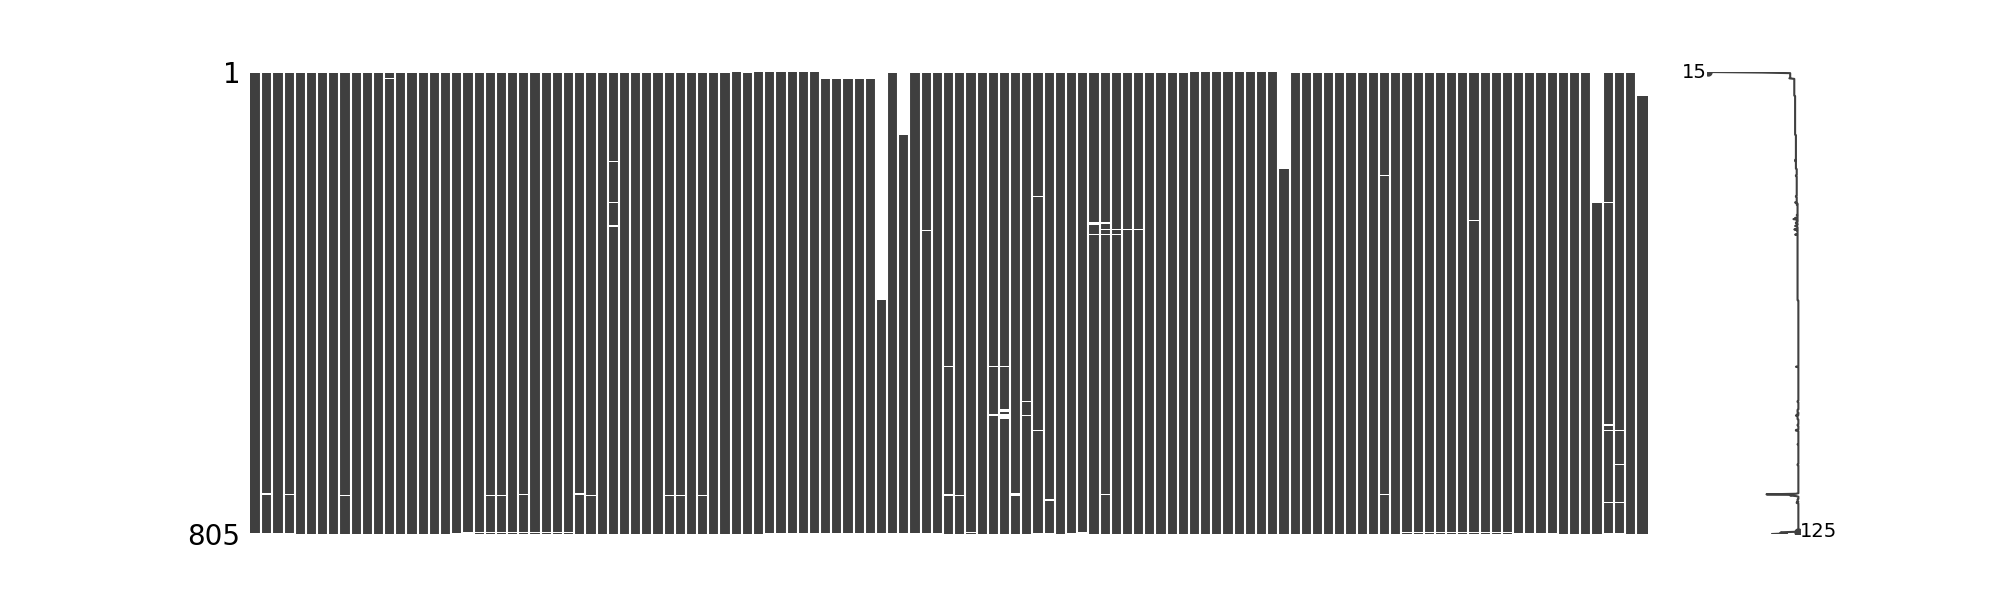
\includegraphics[width=\linewidth]{figures/missing_matrix.png}
    \caption{Missing data matrix for the FRED-MD panel after dropping the four problematic series. Each column is a series; white segments mark missing observations.}
    \label{fig:missing}
\end{figure}
 

\subsection{Stationarity}

The whole panel is made stationary using the FRED-MD recommended transformation codes, mapping each series to their stationary variant. Stationarity ensures that the statistical properties of the series are constant over time, making this step crucial to allow the model to estimate parameters. Indeed, most macroeconomic series are non-stationary in levels.

The two variables to forecast are transformed as follows:
\begin{itemize}
    \item \textbf{INDPRO}: first log-difference, $w_t = \Delta \log \mathrm{INDPRO}_t$, i.e.\ the monthly growth rate of industrial production.
    \item \textbf{PCEPI}: second log-difference, $w_t = \Delta^2 \log \mathrm{PCEPI}_t$, i.e.\ the monthly change in the inflation rate.
\end{itemize}

Figure~\ref{fig:stationary} compares the raw and transformed series for both variables. After transformation, both fluctuate around zero with no visible trend. The choice of second-differencing for PCEPI reflects the fact that inflation itself ($\Delta \log \text{PCEPI}$) still displays persistent dynamics, and a further difference is needed to obtain a clearly mean-stationary series.

\begin{figure}
    \centering
    \begin{subfigure}[t]{0.8\linewidth}
        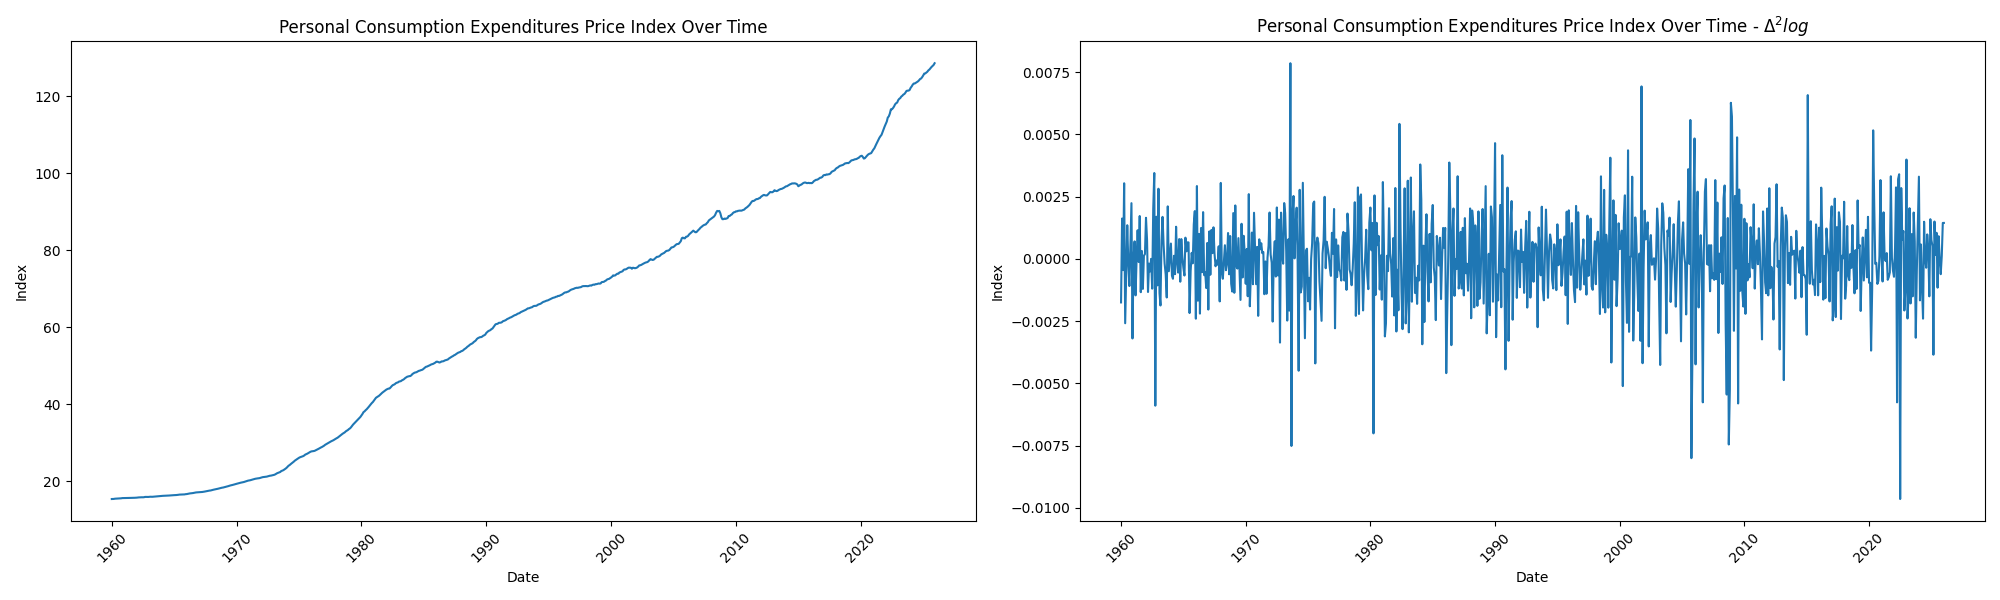
\includegraphics[width=\linewidth]{figures/pcepi_stationary.png}
        \caption{PCEPI: level (left) and $\Delta^2 \log$ (right).}
    \end{subfigure}
    \hfill
    \begin{subfigure}[t]{0.8\linewidth}
        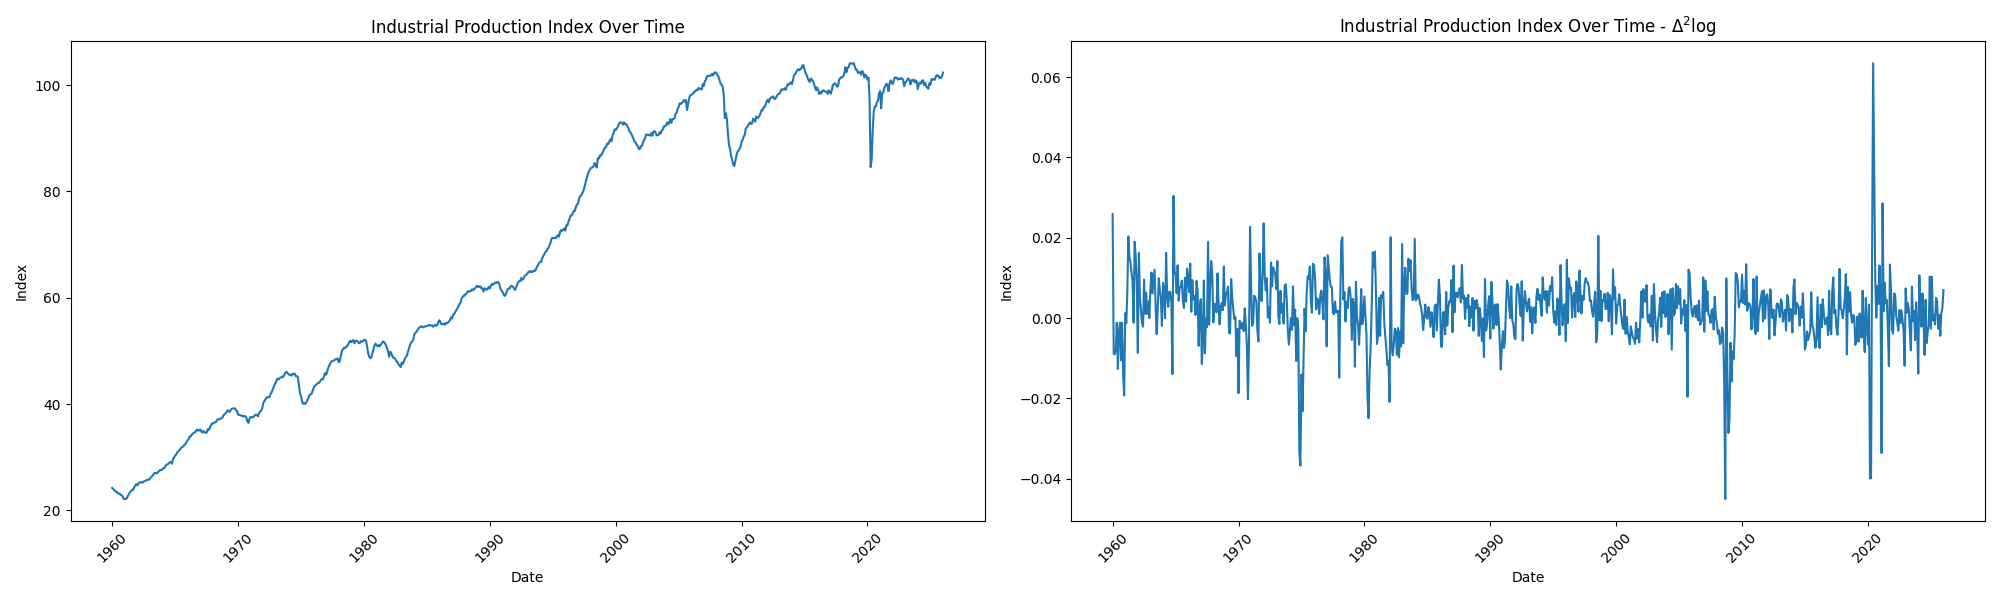
\includegraphics[width=\linewidth]{figures/ipi_stationary.png}
        \caption{INDPRO: level (left) and $\Delta \log$ (right).}
    \end{subfigure}
    \caption{Raw and stationary-transformed target variables.}
    \label{fig:stationary}
\end{figure}

\subsection{Cross-Series Correlation}

Figure~\ref{fig:corr} shows the correlation matrix of the transformed panel. Most pairwise correlations are low, reflecting the breadth of the variables included. A block-diagonal pattern is nonetheless visible: series within the same macroeconomic category tend to move together more than series from different categories. This within-group coherence is what makes dimensionality reduction useful --- a small number of latent common factors may capture a substantial share of the total panel variation.

\begin{figure}[H]
    \centering
    \includegraphics[width=0.65\linewidth]{figures/correlation_matrix.png}
    \caption{Correlation matrix of the stationary FRED-MD panel. Blocks along the diagonal correspond to series within the same macro category.}
    \label{fig:corr}
\end{figure}


% ══════════════════════════════════════════════════════════════════════════════
\section{Methods}
\label{sec:methods}

\subsection{Standardisation}
\label{sec:standardisation}

Before any estimation, all series are standardised on the training sample. Let $Z$ denote the $T \times N$ training matrix and $w$ the $T$-vector of the target variable. For each predictor column $z_i$:
\[
    x_i = \frac{z_i - M_{zi}}{S_{zi}}, \qquad i = 1, \ldots, N,
\]
where $M_{zi}$ and $S_{zi}$ are the sample mean and standard deviation computed on the training window. The target is standardised analogously:
\[
    y = \frac{w - M_w}{S_w}.
\]
The full standardised predictor matrix is $X = (x_1 \cdots x_N)$ of dimension $T \times N$. Standardization is an important prerequisite to make variables comparable, by ensuring that all measures have a common scale. After that a forecast $\hat{y}_{T+1|T}$ is produced in standardised scale it is converted back as $\hat{w}_{T+1|T} = M_w + S_w \cdot \hat{y}_{T+1|T}$.

\subsection{Models}
\label{sec:models}

Eight models are estimated. We distinguish three groups.

\subsubsection*{Autoregressive Models}

Autoregressive models are models where the target variable is regressed on its own past values (lags). The coefficients capture the persistence (memory) of the target variable.

\paragraph{Random Walk (RW)}assumes the next value equals the current one plus a constant drift:
\[
    y_t = \beta_0 + y_{t-1} + e_t.
\]
where $\mathrm{WN}(0,\sigma^2)$ denotes a white noise process with zero mean and constant variance. 

The coefficient on $y_{t-1}$ is set to 1, only $\beta_0$ is estimated by OLS.\footnote{Regressing $\Delta y_t$ on a constant, the OLS estimate reduces to the sample mean of the first differences: $\hat{\beta}_0 = \frac{1}{T-1}\sum_{t=2}^{T}\Delta y_t$.} The forecast is:$\hat{y}_{T+1|T} = \hat{\beta}_0 + y_T.$
While this model is typically suited for non-stationary series, it is included as a naive benchmark and serves as a lower bound for predictive power. Given the standardized and stationary nature of the data, the estimated drift $\hat{\beta}_0$ is expected to be zero, effectively treating the series as a martingale.
\paragraph{AR(1)}
is an autoregressive model with one lag:
\[
    y_t = \beta_0 + \beta_1 y_{t-1} + e_t.
\]
Estimated via OLS. The one-step-ahead forecast is:  $\small \hat{y}_{T+1|T} = \hat{\beta}_0 + \hat{\beta}_1 y_T.$
The coefficient $\beta_1$ captures the degree of persistence in the series. Differently from the RW (where $\beta_1 = 1$), AR models account for the mean-reverting nature of the data: while shocks may have a lasting effect, their effect eventually decay if $|\beta| < 1$. Otherwise, if $\beta_1 \geq 1$, the series would have an explosive behavior.

\paragraph{AR($p$)} is a general autoregressive model:
\[
    y_t = \beta_0 + \beta_1 y_{t-1} + \cdots + \beta_p y_{t-p} + e_t.
\]
Estimated via OLS. The one-step-ahead forecast is:  $\small \hat{y}_{T+1|T} = \hat{\beta}_0 + \hat{\beta}_1 y_T + \cdots + \hat{\beta}_p y_{T-p+1}$.
The AR(p) model expads on the AR(1) to capture more complex lag dynamics. In this case, stationarity requires $|\sum_{i=1}^p \beta_i| < 1$. The lag order $p$ is selected by BIC (see Section~\ref{sec:tuning}).


\subsubsection*{Multivariate Models}

These models incorporate the full lagged predictor matrix $X_{t-1}$. The general specification is:
\[
    y_t = \beta_0 + X'_{t-1}\beta + e_t, \qquad t = 2,\ldots,T,
\]
where $X_{t-1}$ is the $(N-1)$-vector of predictors at time $t-1$. The one-step-ahead forecast is:  $\small \hat{y}_{T+1|T} = \hat{\beta}_0 + X'_T\hat{\beta}$.

\paragraph{OLS}
is an unconstrained least squares regression. When the number of variables is close to the number of observations, OLS introduces the curse of dimensionality, i.e. issues related to high-dimensional spaces, including the risk of overfitting. For this reason, shrinkage methods like Ridge and Lasso are introduced.

\paragraph{Ridge} adds an $\ell_2$ penalty on the coefficient vector, i.e. imposes an upper bound on the sum of squared coefficients:
\[
    \hat{\beta}^{\text{ridge}} = \operatorname*{arg\,min}_\beta \Bigl\{ \|y - X\beta\|^2 + \lambda\|\beta\|^2 \Bigr\}.
\]
Larger $\lambda$ shrinks all coefficients closer to zero, but no coefficient is ever set exactly to zero.
The closed-form solution is:  $\small \hat{\beta}^{\text{ridge}} = (X'X + \lambda I)^{-1}X'y$, which is always well-defined regardless of the rank of $X'X$.

\paragraph{Lasso} uses an $\ell_1$ norm (sum of absolute values of coefficients):
\[
    \hat{\beta}^{\text{lasso}} = \operatorname*{arg\,min}_\beta \Bigl\{ \|y - X\beta\|^2 + \lambda\|\beta\|_1 \Bigr\}.
\]
Lasso potentially performs variable selection: as  $\lambda$ increases, some coefficients are driven to zero, introducing sparsity.

There is no closed-form solution for Lasso; the problem is solved via coordinate descent. The forecast is:  $\small \hat{y}_{T+1|T} = \hat{\beta}^{\text{lasso}}_0 + X'_T\hat{\beta}^{\text{lasso}}.$

\subsubsection*{Principal Component Regression (PCR)}

PCA is applied to $X$ to extract a small number of linear combinations of the original predictors that summarise most of the panel's variation. Concretely, the $k$-th principal component is $\hat{F}_{kt} = X_t v_k$, where $v_k$ is the $k$-th eigenvector of $X'X$ (ordered by decreasing eigenvalue). Each $\hat{F}_{kt}$ is therefore a weighted average of the $N$ standardised predictors at time $t$, with weights chosen to maximise explained variance. The $r$ leading components are collected into a vector $\hat{F}_t = (\hat{F}_{1t}, \ldots, \hat{F}_{rt})'$.
 These $r$ components replace the original $N$ predictors in the regression:
\[
    y_t = \beta_0 + \hat{F}'_{t-1}\beta + e_t.
\]
Estimated by OLS. The forecast is:  $ \small \hat{y}_{T+1|T} = \hat{\beta}_0 + \hat{F}'_T\hat{\beta}.$

\subsection{Hyperparameter Tuning}
\label{sec:tuning}

The AR lag order, the Ridge and Lasso penalties are selected using data from the first training window only and are then held fixed throughout the expanding-window forecast. This choice avoids the look-ahead bias that would arise from cross-validation on more windows, is less computationally intensive, and also better simulates an actual real-time setup.

Selection is based on the Bayesian Information Criterion (BIC):
\[
    \mathrm{BIC} = n\log(\hat{\sigma}^2) + k\log(n),
\]
where $n$ is the number of observations used in estimation, $k$ is the effective number of parameters, and $\hat{\sigma}^2$ is the residual variance. BIC penalises model complexity more heavily than AIC, which tends to produce more parsimonious selections.

The number of principal components is selected looking for the elbow in the eigenvalue distribution (Figure~\ref{fig:pca_scree}), which describes the proportion of variance explained by each component.

\subsection{Forecasting Framework and Evaluation}
\label{sec:framework}

The forecast -- or model evaluation -- follows an expanding-window out-of-sample design. The total sample has $T_1$ observations; the first $T \approx \tfrac{2}{3} T_1$ form the first training window, and the remaining $T_1 - T$ observations constitute the evaluation period. The sample provides 787 data points, of which 263 are used for evaluation. At each step $t = T, T+1, \ldots, T_1 - 1$:
\begin{enumerate}
    \item Each model is estimated on observations $1, \ldots, t$.
    \item A one-step-ahead forecast $\hat{w}_{t+1|t}$ is produced in standardised, transformed scale and then converted to the original level:
          \begin{itemize}
              \item \textbf{INDPRO}: $\widehat{\mathrm{INDPRO}}_{t+1|t} = \exp\!\bigl(\log \mathrm{INDPRO}_t + \hat{w}_{t+1|t}\bigr)$
              \item \textbf{PCEPI}: $\log\widehat{\mathrm{PCEPI}}_{t+1|t} = \hat{w}_{t+1|t} + 2\log\mathrm{PCEPI}_t - \log\mathrm{PCEPI}_{t-1}$
          \end{itemize}
    \item The window expands by one observation.
\end{enumerate}

Models are compared using the Root Mean Squared Error:
\[
    \mathrm{RMSE} = \sqrt{\frac{1}{T_1 - T}\sum_{t=T}^{T_1 - 1}\bigl(\hat{y}_{t+1|t} - y_{t+1}\bigr)^2}.
\]


% ══════════════════════════════════════════════════════════════════════════════
\section{Results}
\label{sec:results}

\subsection{Hyperparameter Tuning}
\label{sec:res_tuning}

\subsubsection*{AR Lag Order}

BIC selects $p = 3$ for INDPRO and $p = 5$ for PCEPI. The objective of the AR model is to capture the serial autocorrelation of the target variable, so that only uncorrelated white noise is left in the residuals. Indeed, Figure~\ref{fig:ar_acf} shows that, using these lag orders, the ACF of AR residuals on the first training window is not statistically significant.
Figure~\ref{fig:acf} shows that the original series display a clear autocorrelation in the first lags. While the BIC criterion might seem surprising given the raw ACF, its partial autocorrelation (PACF) (Figure~\ref{fig:pacf}) confirms that INDPRO requires a different number of lags to fully whiten residuals. \footnote{The PACF at lag $k$ measures the correlation between $y_t$ and $y_{t-k}$ after removing the linear contribution of the intermediate lags $1,\ldots,k-1$.}
\begin{figure}[H]
    \centering
    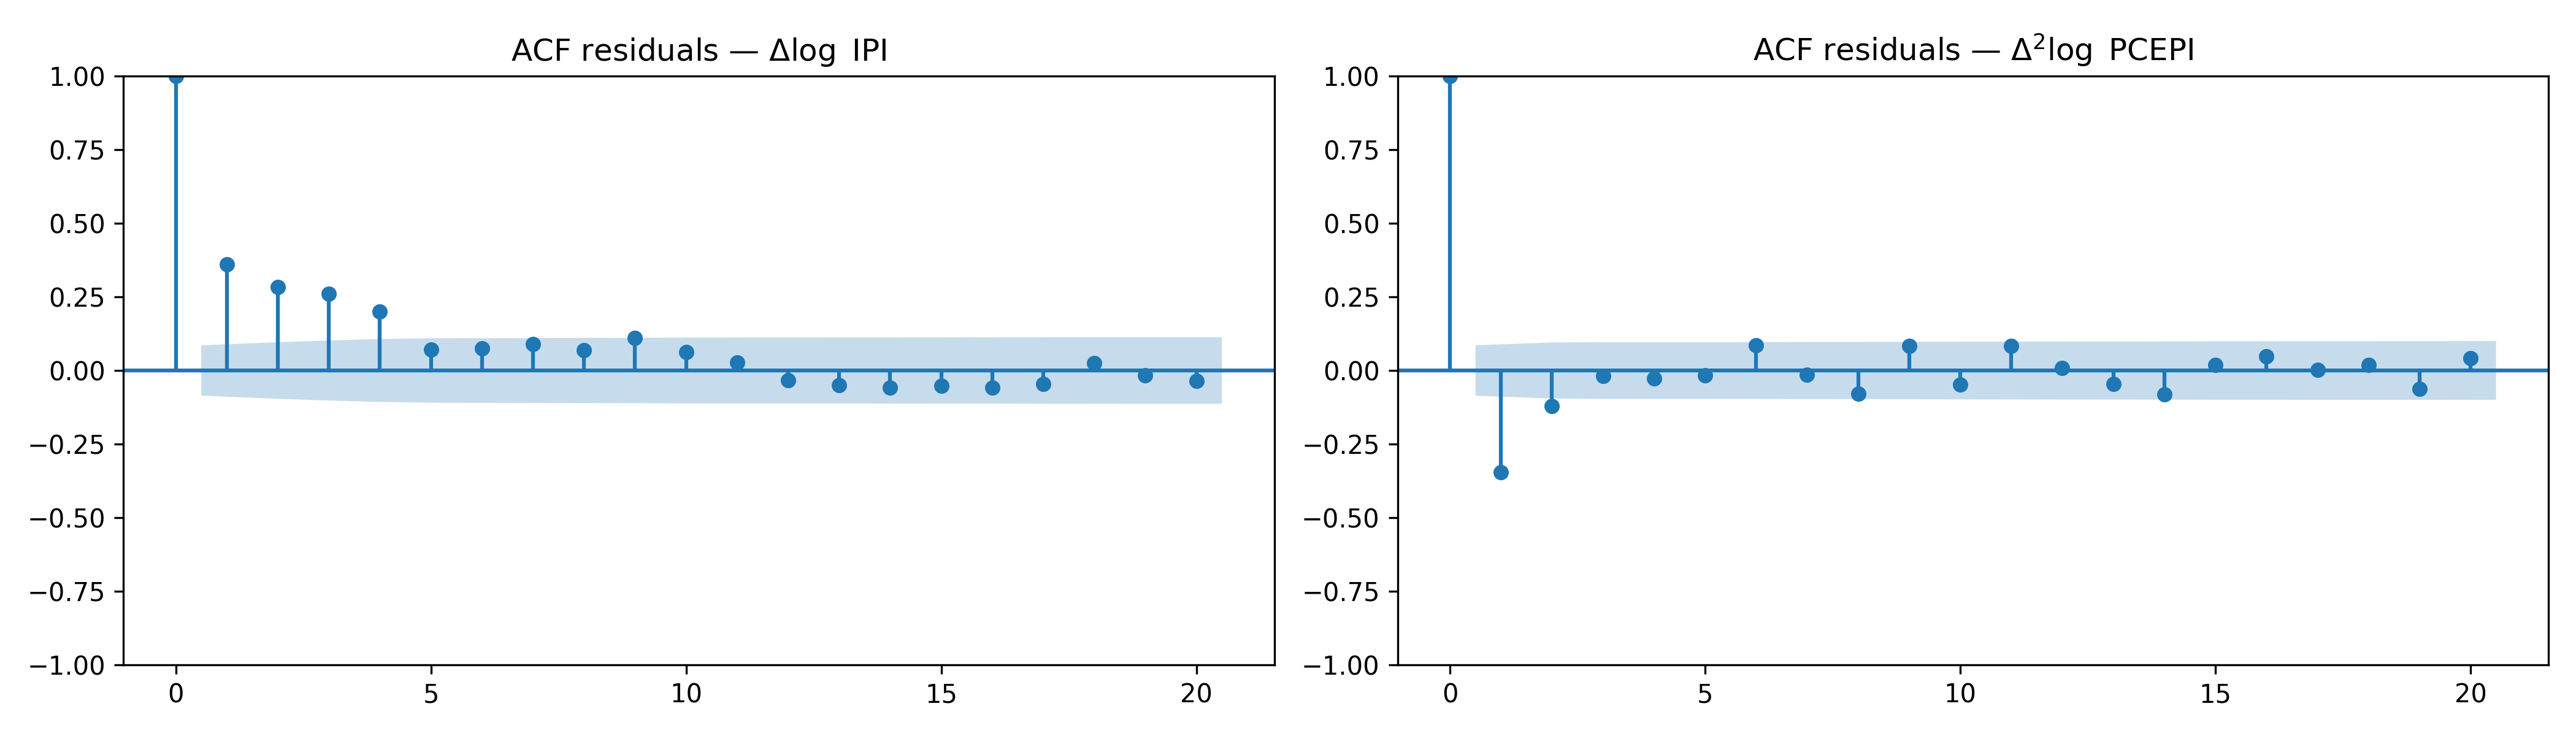
\includegraphics[width=0.9\linewidth]{figures/acf.png}
    \caption{ACF of AR residuals on the first training window. Left: INDPRO. Right: PCEPI.}
    \label{fig:acf}
\end{figure}


\begin{figure}[H]
    \centering
    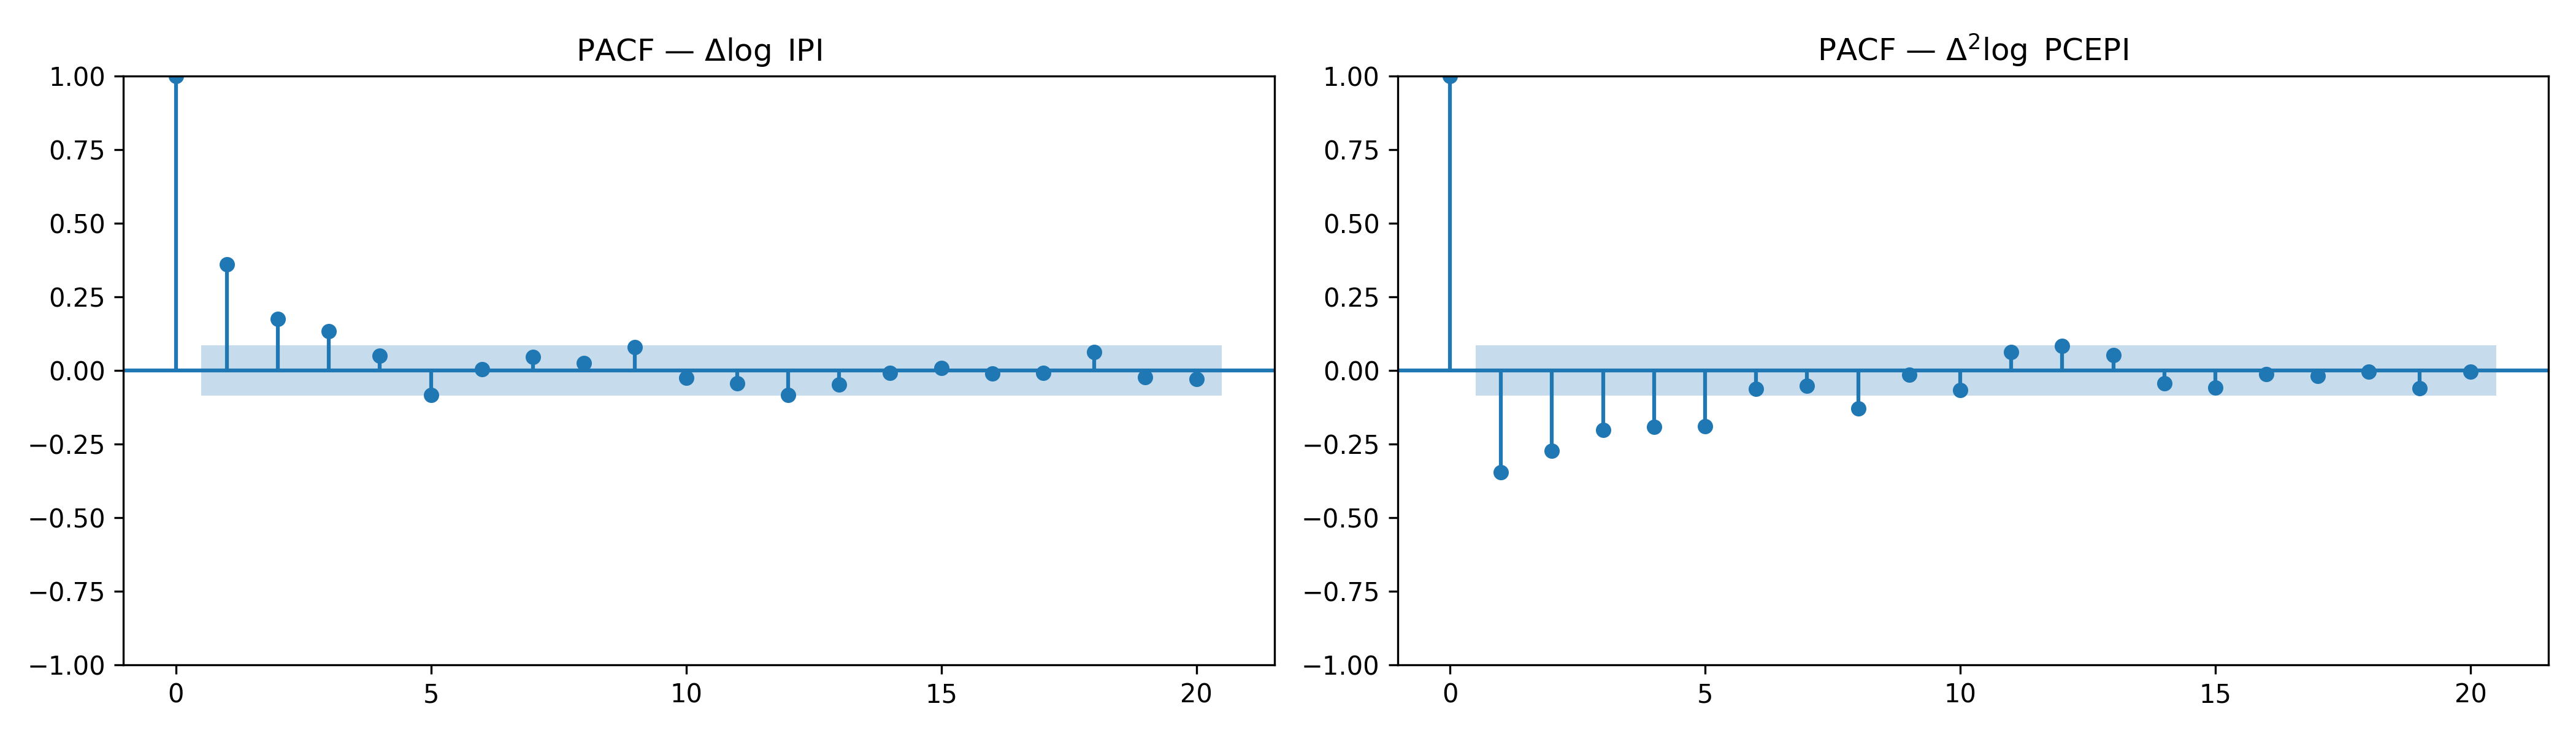
\includegraphics[width=0.9\linewidth]{figures/pacf.png}
    \caption{PACF of AR residuals on the first training window. Left: INDPRO. Right: PCEPI.}
    \label{fig:pacf}
\end{figure}


\begin{figure}[H]
    \centering
    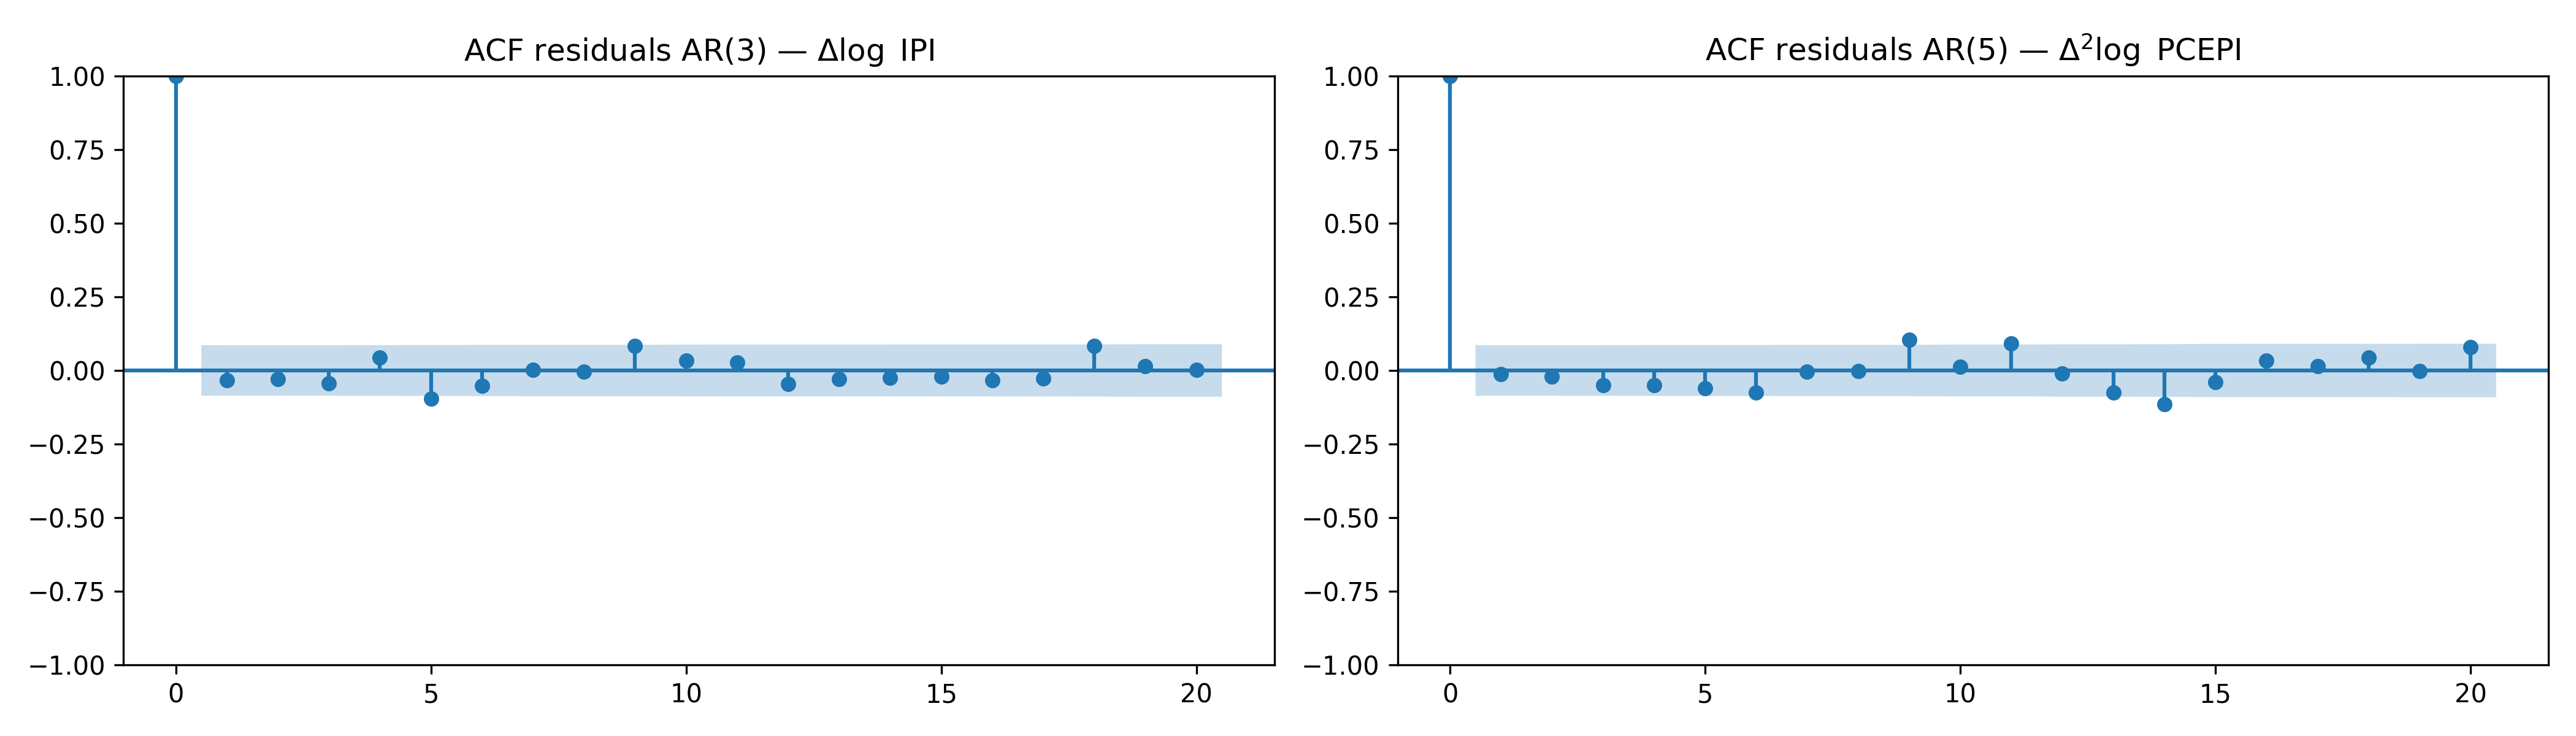
\includegraphics[width=0.9\linewidth]{figures/ar_residuals_acf.png}
    \caption{ACF of AR residuals on the first training window. Left: INDPRO. Right: PCEPI.}
    \label{fig:ar_acf}
\end{figure}

\subsubsection*{Penalisation Hyperparameters}

Figure~\ref{fig:bic} shows the BIC curves over the penalisation grid for Ridge and Lasso.

\begin{figure}[H]
    \centering
    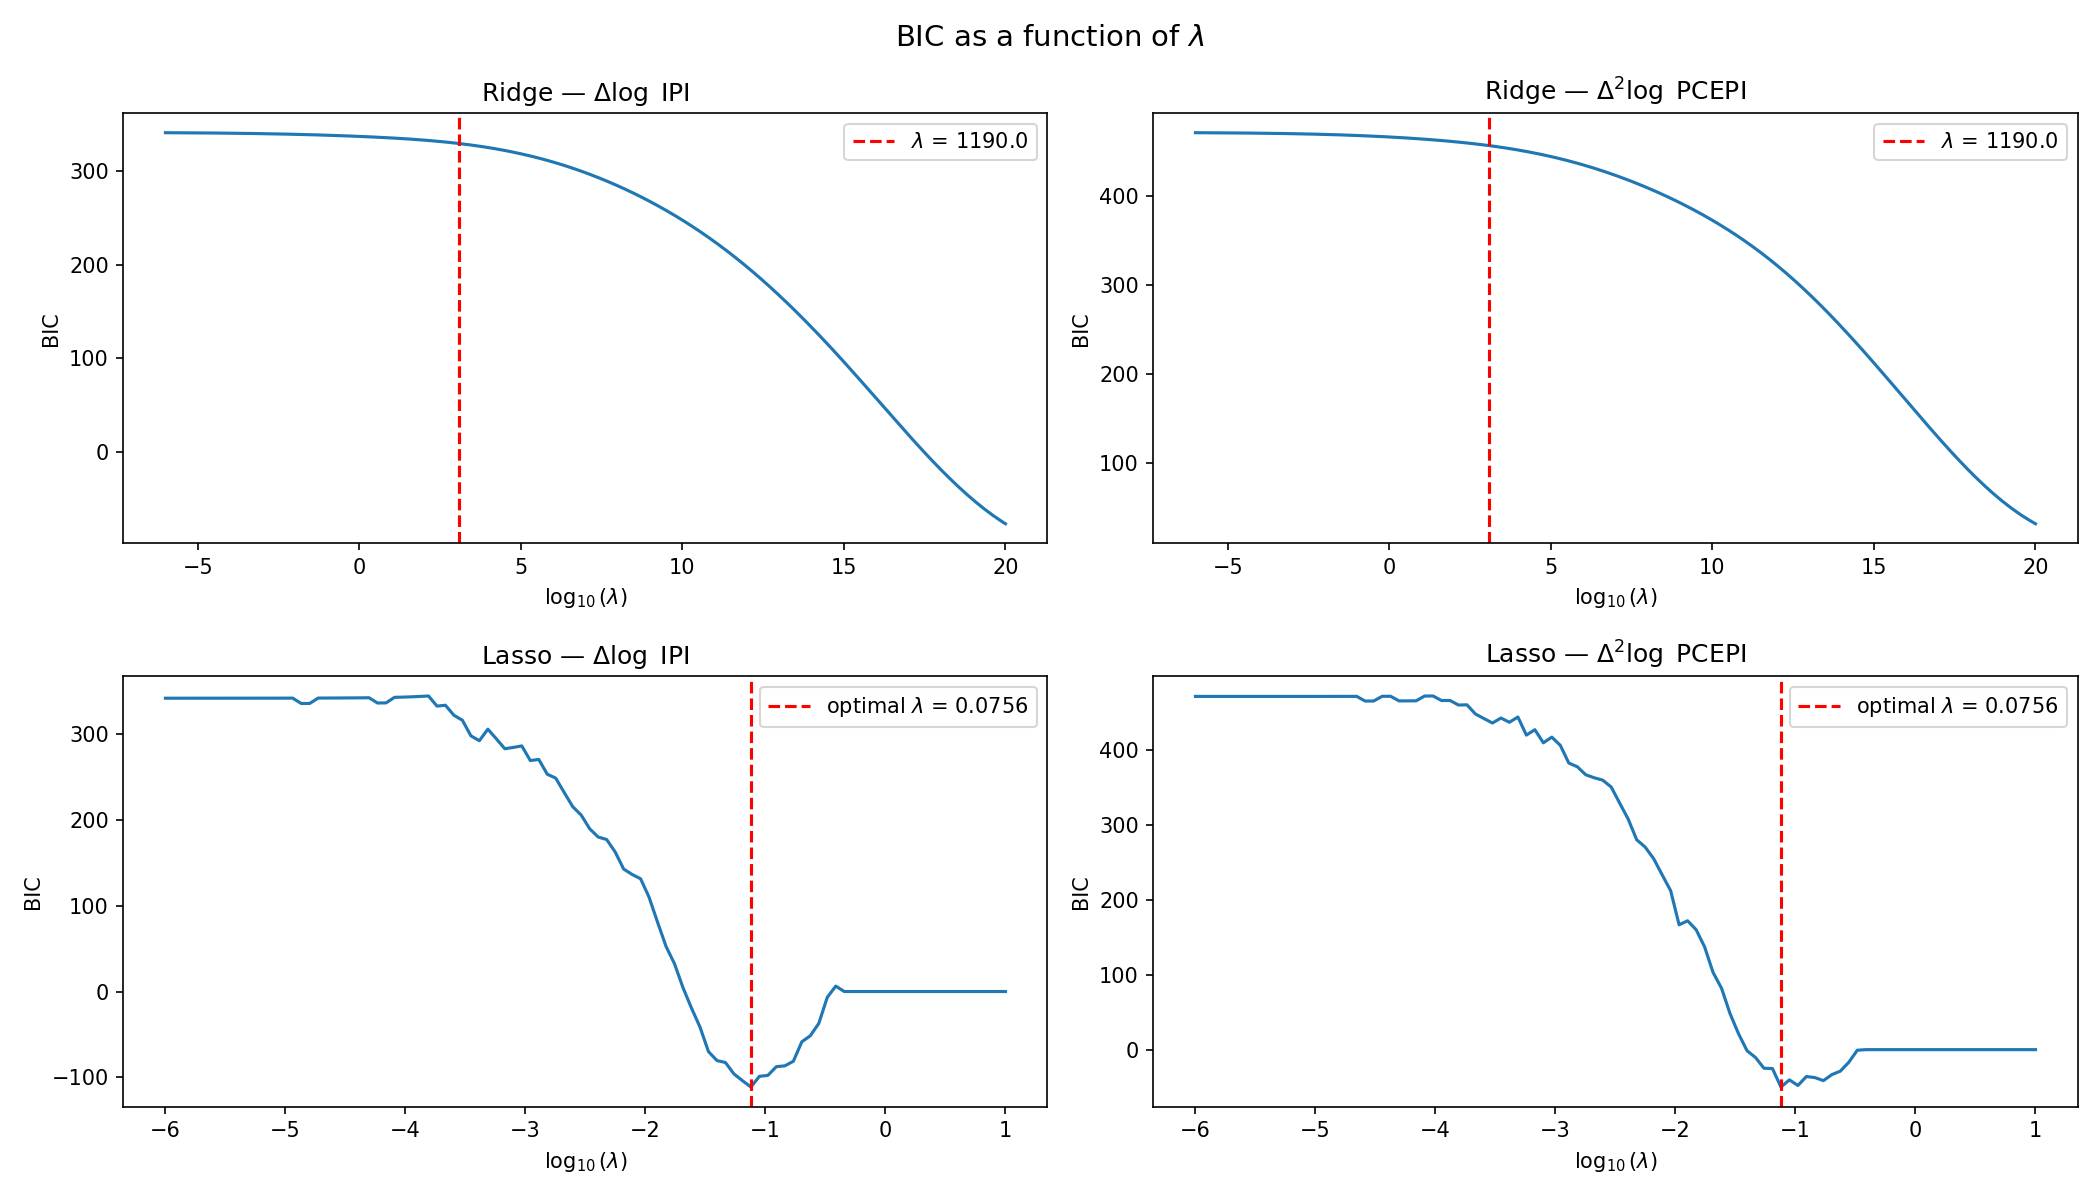
\includegraphics[width=\linewidth]{figures/bic_comparison.png}
    \caption{BIC as a function of $\lambda$ for Ridge and Lasso, separately for INDPRO and PCEPI. Red dashed lines mark the selected value.}
    \label{fig:bic}
\end{figure}

The Ridge BIC decreases monotonically across the entire grid, with no interior minimum. This indicates that the model consistently favours stronger shrinkage, a pattern that might be justified by the mild correlation with most variables. De Mol et al.\ (2008) suggest that a reasonable range is $[0.5N , 10N]$, therefore we fix $\lambda_{\text{ridge}} = 1190$, to the upper bound of this range.
The Lasso BIC, by contrast, has a well-defined minimum, identifying a specific optimal penalty. At the selected $\lambda$, Lasso retains 17 non-zero coefficients for INDPRO and 9 for PCEPI out of 119 total predictors. This suggests that a sparse model is more adequate for inflation than industrial production.


Figure~\ref{fig:coef_paths} shows the full regularisation paths.

\begin{figure}[H]
    \centering
    \begin{subfigure}[t]{0.85\linewidth}
        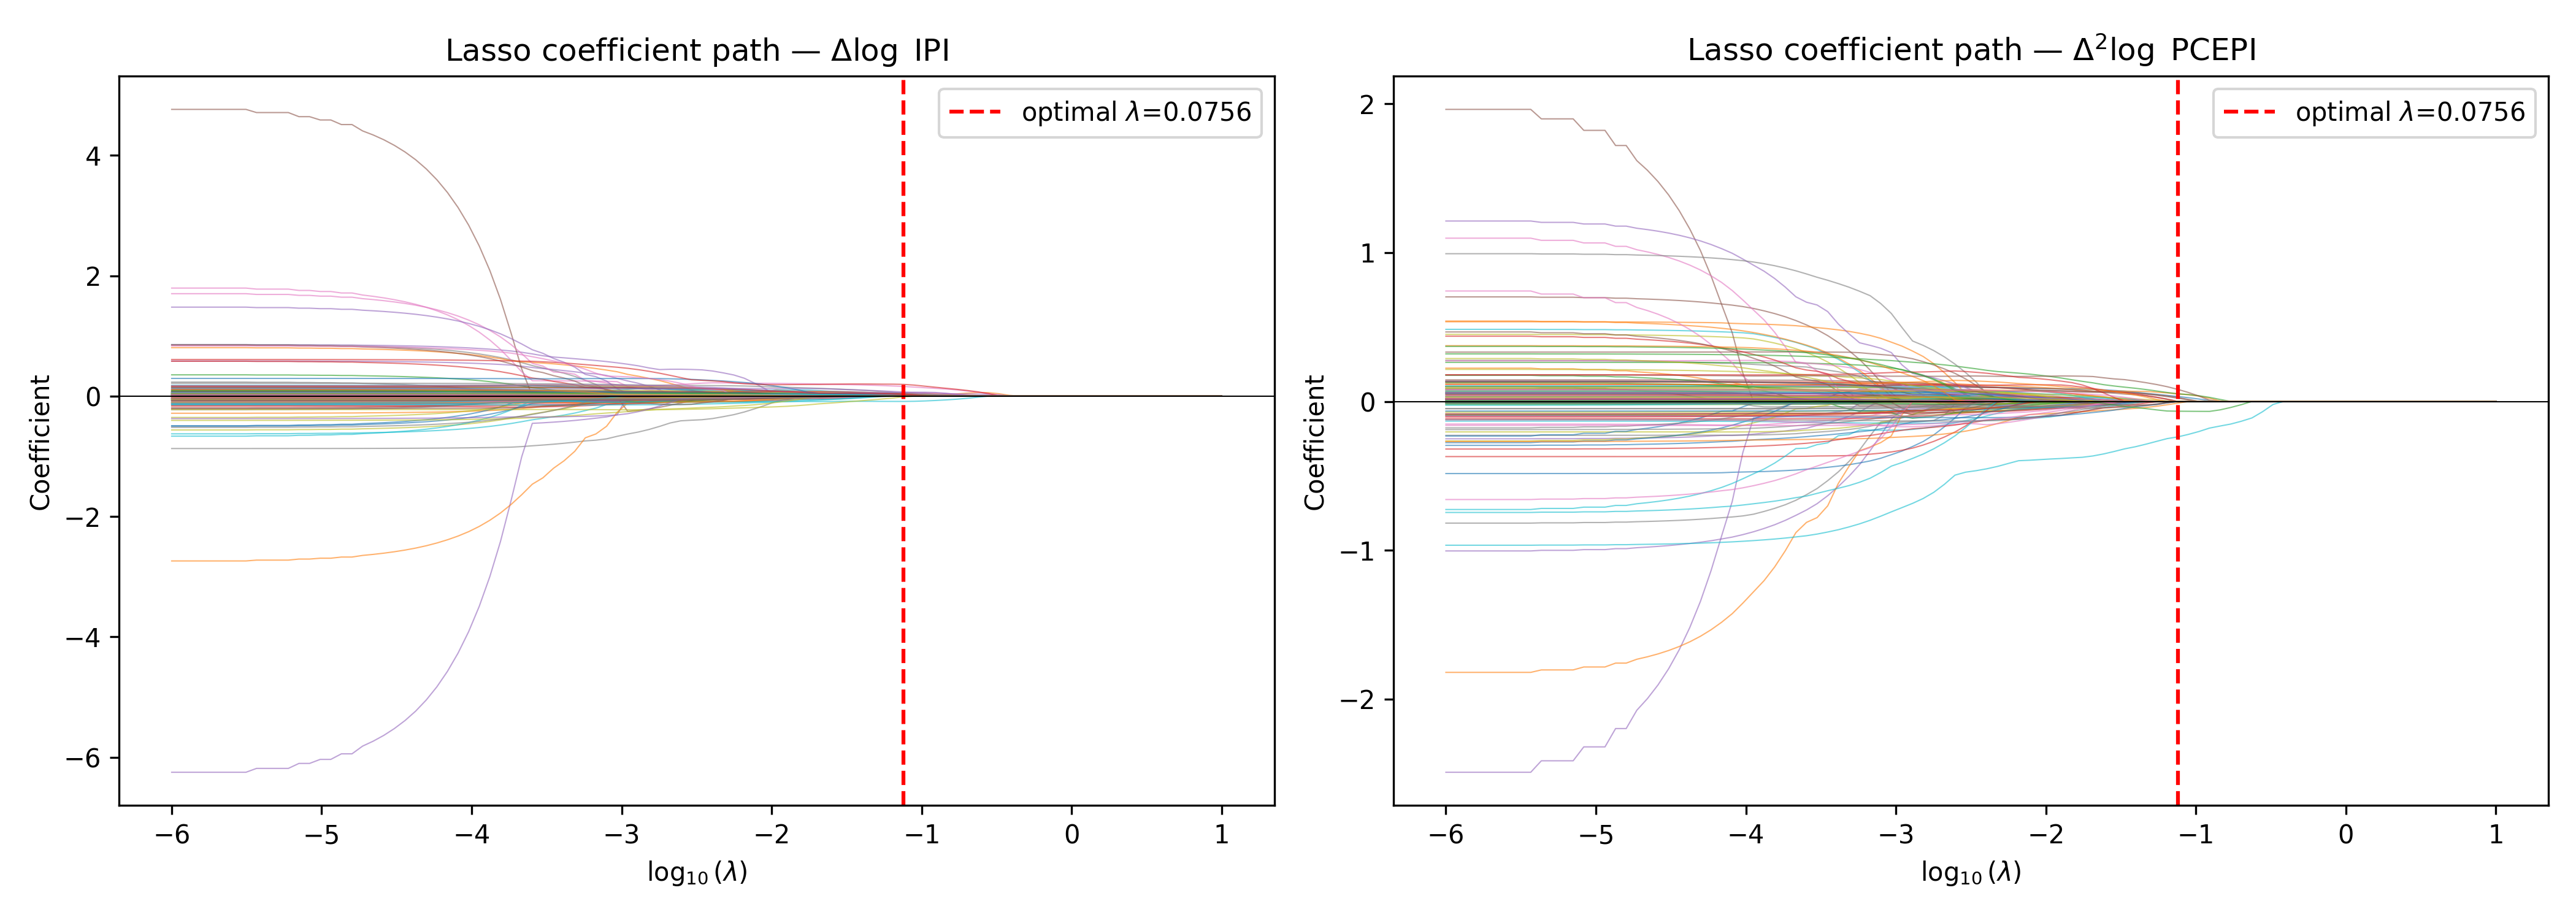
\includegraphics[width=\linewidth]{figures/lasso_coef_path.png}
        \caption{Lasso paths.}
    \end{subfigure}
    \hfill
    \begin{subfigure}[t]{0.85\linewidth}
        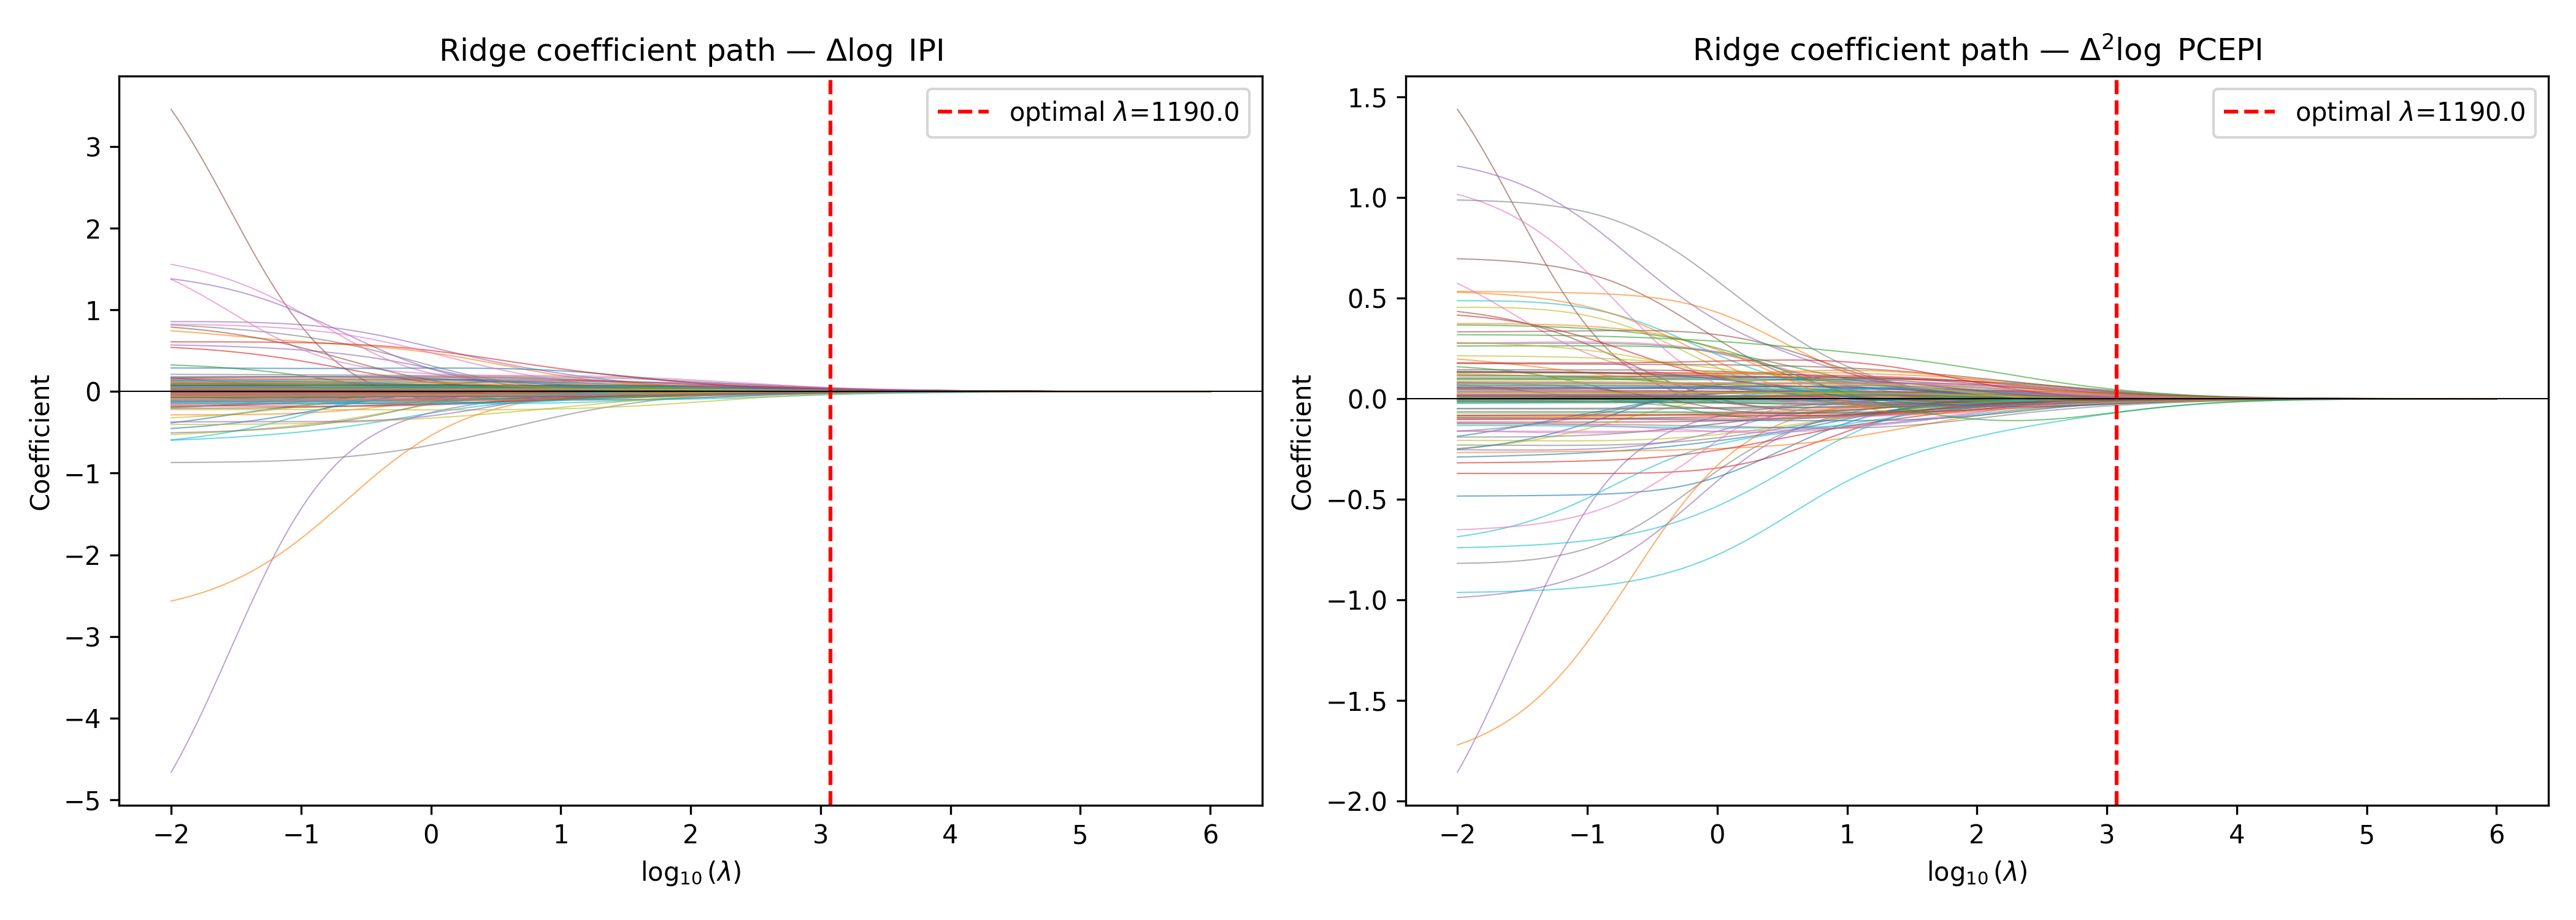
\includegraphics[width=\linewidth]{figures/ridge_coef_path.png}
        \caption{Ridge paths.}
    \end{subfigure}
    \caption{Coefficient regularisation paths as a function of $\log_{10}(\lambda)$. Red dashed line: BIC-selected penalty.}
    \label{fig:coef_paths}
\end{figure}

Tables 1 and 2 report the variables selected by Lasso for IPI and CPI respectively, along with their coefficients. Since both target variables are transformed to stationarity, coefficients reflect the contribution of each predictor to the growth rate of industrial production and to the acceleration of inflation, not to their levels.
A notable asymmetry concerns the selection of own lags. For IPI, Lasso does not select any lag of INDPRO itself, favouring instead external labour market and real-side predictors. For CPI, by contrast, PCEPI enters with a negative coefficient ($-0.238$): since the target is transformed to second log-difference, this reflects mean reversion in inflation acceleration --- above-average price growth at $t-1$ tends to be partially offset at $t$.
For IPI, Lasso selects variables from the labour market and housing sectors, alongside interest rate spreads, which capture credit conditions. No price variables are selected, consistent with industrial production being primarily driven by real-side dynamics. For CPI, the model selects a mix of variables that capture different sources of inflationary pressure: real PCE and personal income reflect demand conditions, monetary aggregates (M2, non-borrowed reserves) capture the role of money supply, and the PPI for finished goods proxies increasing cost pressures.


{%
\setlength{\floatsep}{6pt plus 1pt minus 1pt}
\setlength{\textfloatsep}{6pt plus 1pt minus 1pt}
\begin{table}[H]
\centering
\caption{Lasso selected predictors — IPI (17/119 non-zero)}
\begin{tabular}{llrl}
\toprule
Variable & Description & Coef & Group \\
\midrule
CLAIMSx        & Initial Unemployment Insurance Claims      & $-0.088$ \\
BUSINVx        & Total Business Inventories                 & $-0.012$ \\
AAA            & Moody's Aaa Corporate Bond Yield           & $+0.013$ \\
HWIURATIO      & Help Wanted / Unemployment                 & $+0.015$ \\
HWI            & Help Wanted Index                          & $+0.018$ \\
USTPU          & Employees: Trade, Transport \& Utilities   & $+0.022$ \\
CES0600000008  & Avg Hourly Earnings: Goods-Producing       & $+0.027$ \\
HOUSTS         & Housing Starts: South                      & $+0.033$ \\
FEDFUNDS       & Effective Federal Funds Rate               & $+0.034$ \\
HOUST          & Housing Starts: Total                      & $+0.034$ \\
USTRADE        & Employees: Retail Trade                    & $+0.035$ \\
AMDMUOx        & Unfilled Orders: Durable Goods             & $+0.049$ \\
IPMAT          & IP: Materials                              & $+0.049$ \\
CP3Mx          & 3-Month Commercial Paper Rate              & $+0.061$ \\
CES2000000008  & Avg Hourly Earnings: Construction          & $+0.066$ \\
NDMANEMP       & Employees: Non-durable Goods Mfg           & $+0.160$ \\
TB3SMFFM       & 3-Month T-Bill minus Fed Funds             & $+0.195$ \\
\bottomrule
\end{tabular}
\end{table}

\vspace{-0.3em}
\begin{table}[H]
\centering
\caption{Lasso selected predictors — CPI (9/119 non-zero)}
\begin{tabular}{llrl}
\toprule
Variable & Description & Coef & Group \\
\midrule
PCEPI              & PCE Price Index (lagged)               & $-0.238$ \\
DSERRG3M086SBEA    & Real PCE: Services                     & $-0.066$ \\
S\&P div yield     & S\&P 500 dividend yield                & $-0.011$ \\
IPB51222S          & IP: Nondurable Energy Consumer Goods         & $+0.022$ \\
NONBORRES          & Non-borrowed Reserves                  & $+0.027$ \\
W875RX1            & Real Personal Income ex.\ Transfers    & $+0.033$ \\
DPCERA3M086SBEA    & Real PCE                               & $+0.051$ \\
M2REAL             & Real M2 Money Stock                    & $+0.051$ \\
WPSFD49502         & PPI: Finished Consumer Goods ex.\ Food & $+0.081$ \\
\bottomrule
\end{tabular}
\end{table}
}


\subsubsection*{Principal Components}

Figure~\ref{fig:pca_scree} shows the scree plot; the elbow corresponds to $r = 6$ principal components, explaining approximately 60\% of the total panel variance.

\begin{figure}[H]
    \centering
    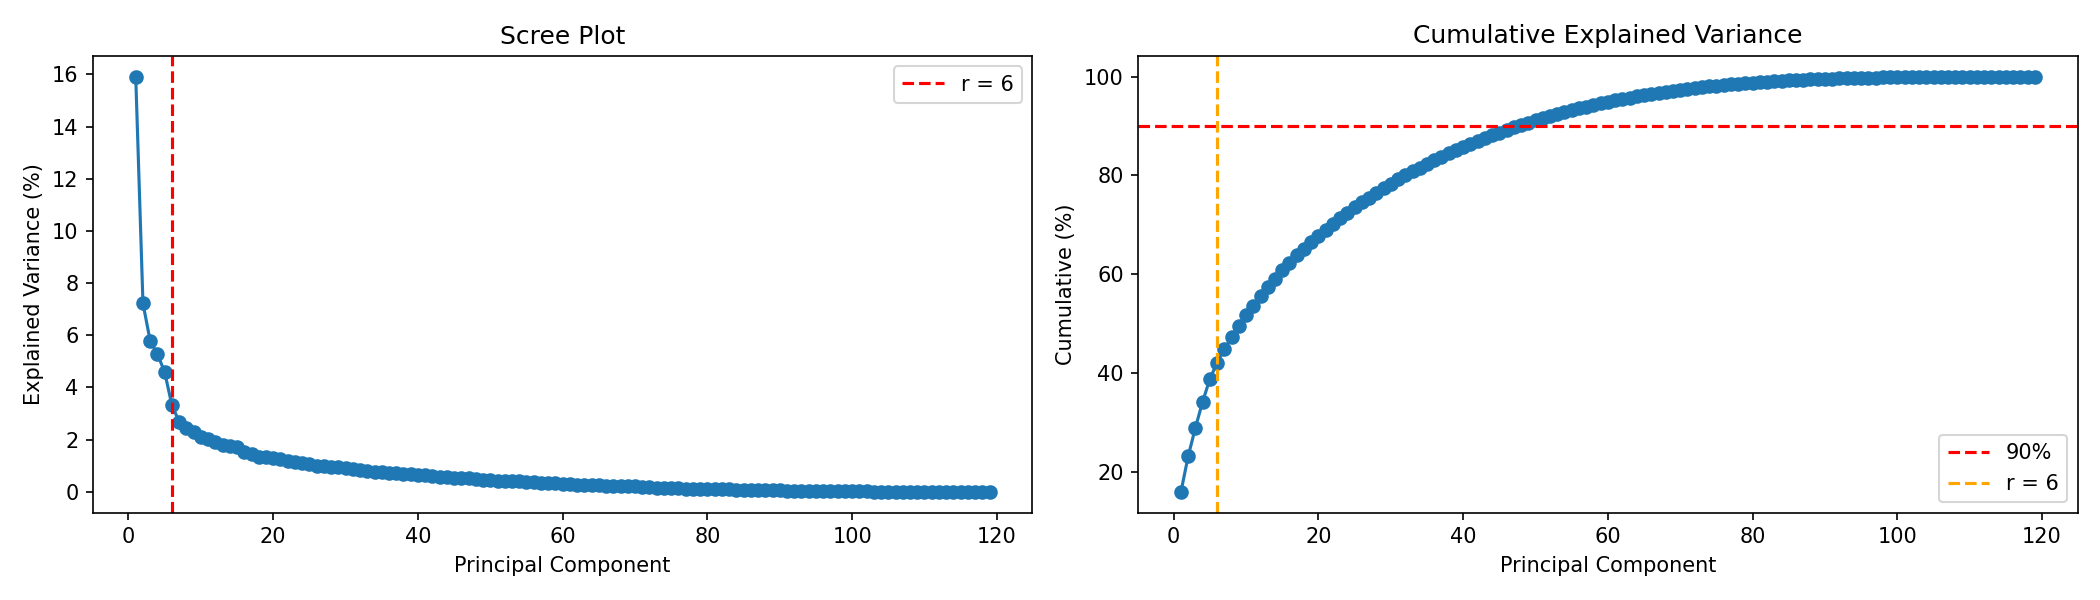
\includegraphics[width=0.85\linewidth]{figures/pca_scree.png}
    \caption{Scree plot of eigenvalues. Elbow at $r = 6$, explaining roughly 60\% of total panel variance.}
    \label{fig:pca_scree}
\end{figure}

Figure~\ref{fig:pca_comp} shows the first six principal components over time, with the NBER recession periods shaded in grey. McCracken \& Ng provide an interpretation of the first components: PC 1 can be interpreted as a real activity and employment factor, PC 2 represents a forward-looking factor, driven by variables such as term interest rate spreads and inventories. PC 3 corresponds to an inflation factor, while Factors 4 and 5 combine housing and interest rate elements. Finally, PC 6, like PC 1, is primarily associated with real activity and employment.
\begin{figure}[H]
    \centering
    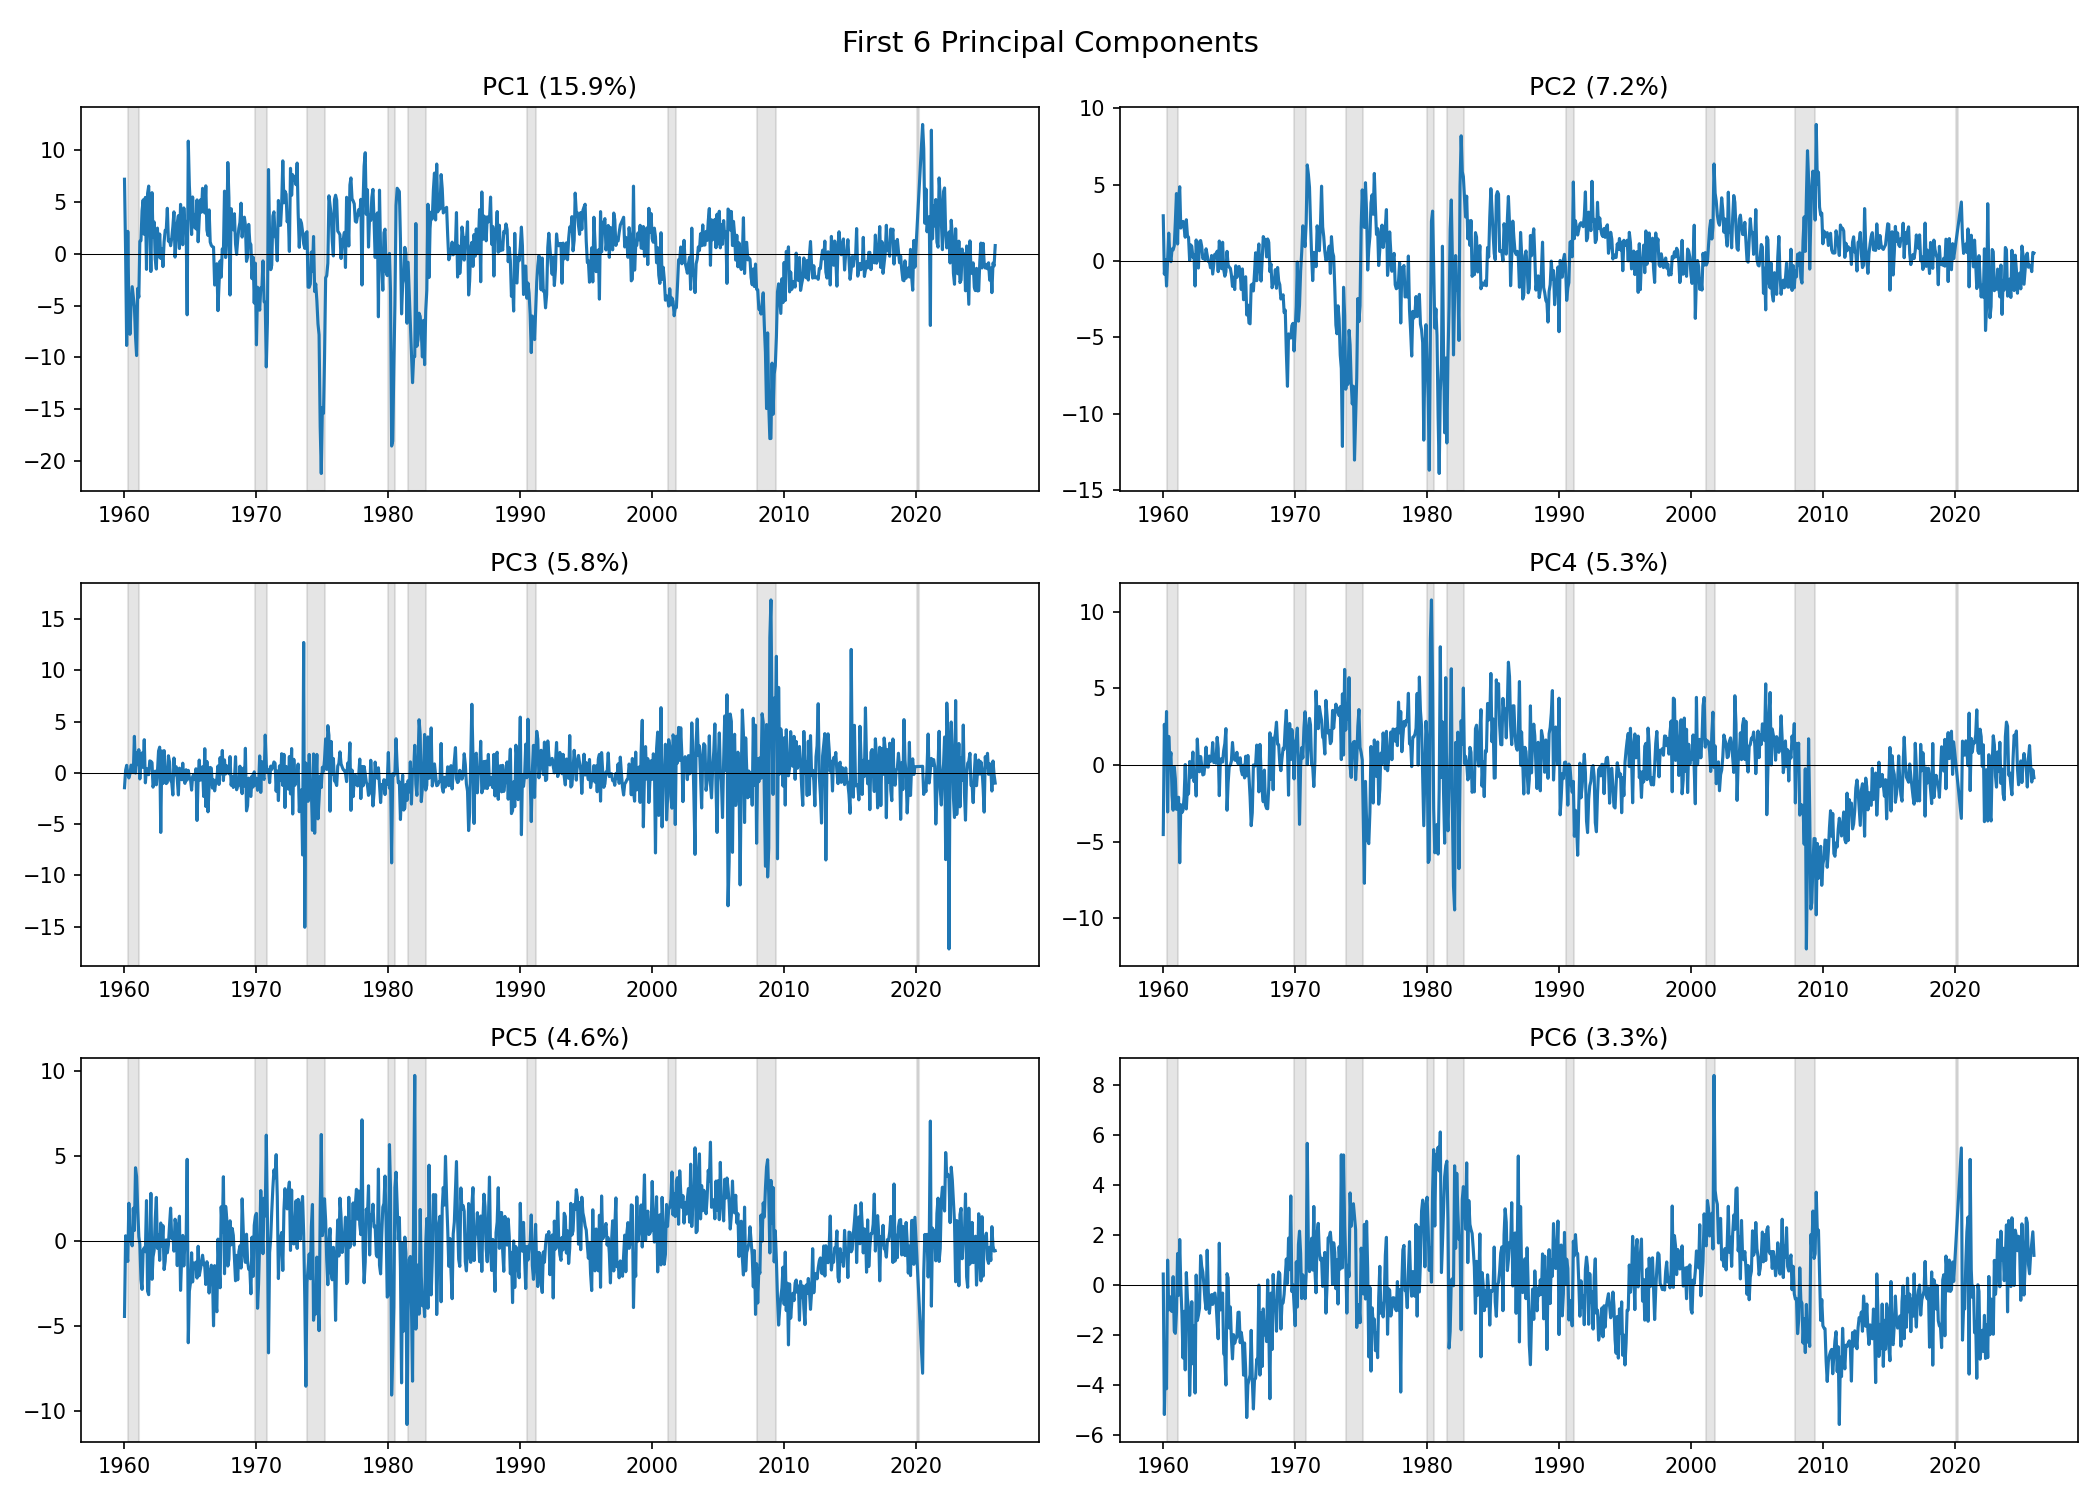
\includegraphics[width=\linewidth]{figures/pca_components.png}
    \caption{First six principal components of the standardised FRED-MD panel over time.}
    \label{fig:pca_comp}
\end{figure}
 
\subsection{Forecast Results}
\label{sec:res_forecast}

Figure~\ref{fig:ipi_forecasts} and Figure~\ref{fig:pcepi_forecasts} show the expanding-window forecasts against actual values in transformed scale, grouped by model family.
In transformed scale, AR models produce smoother forecasts than the Random Walk, reflecting lower estimated persistence: since $\hat\beta_1 < 1$, shocks decay rather than propagate one-for-one. Among multivariate models, Ridge and Lasso appear overall less volatile than OLS: the shrinkage penalty effectively damps the forecast path by lowering the magnitude of coefficients. For PCEPI, PCR1 produces a nearly flat forecast. This might be due both to the fact that the first principal component is chiefly related to real activity, which might be less relevant to inflation forecast (as highlighted by the Lasso selection), and to the transformation to second difference.

\begin{figure}[H]
    \centering
    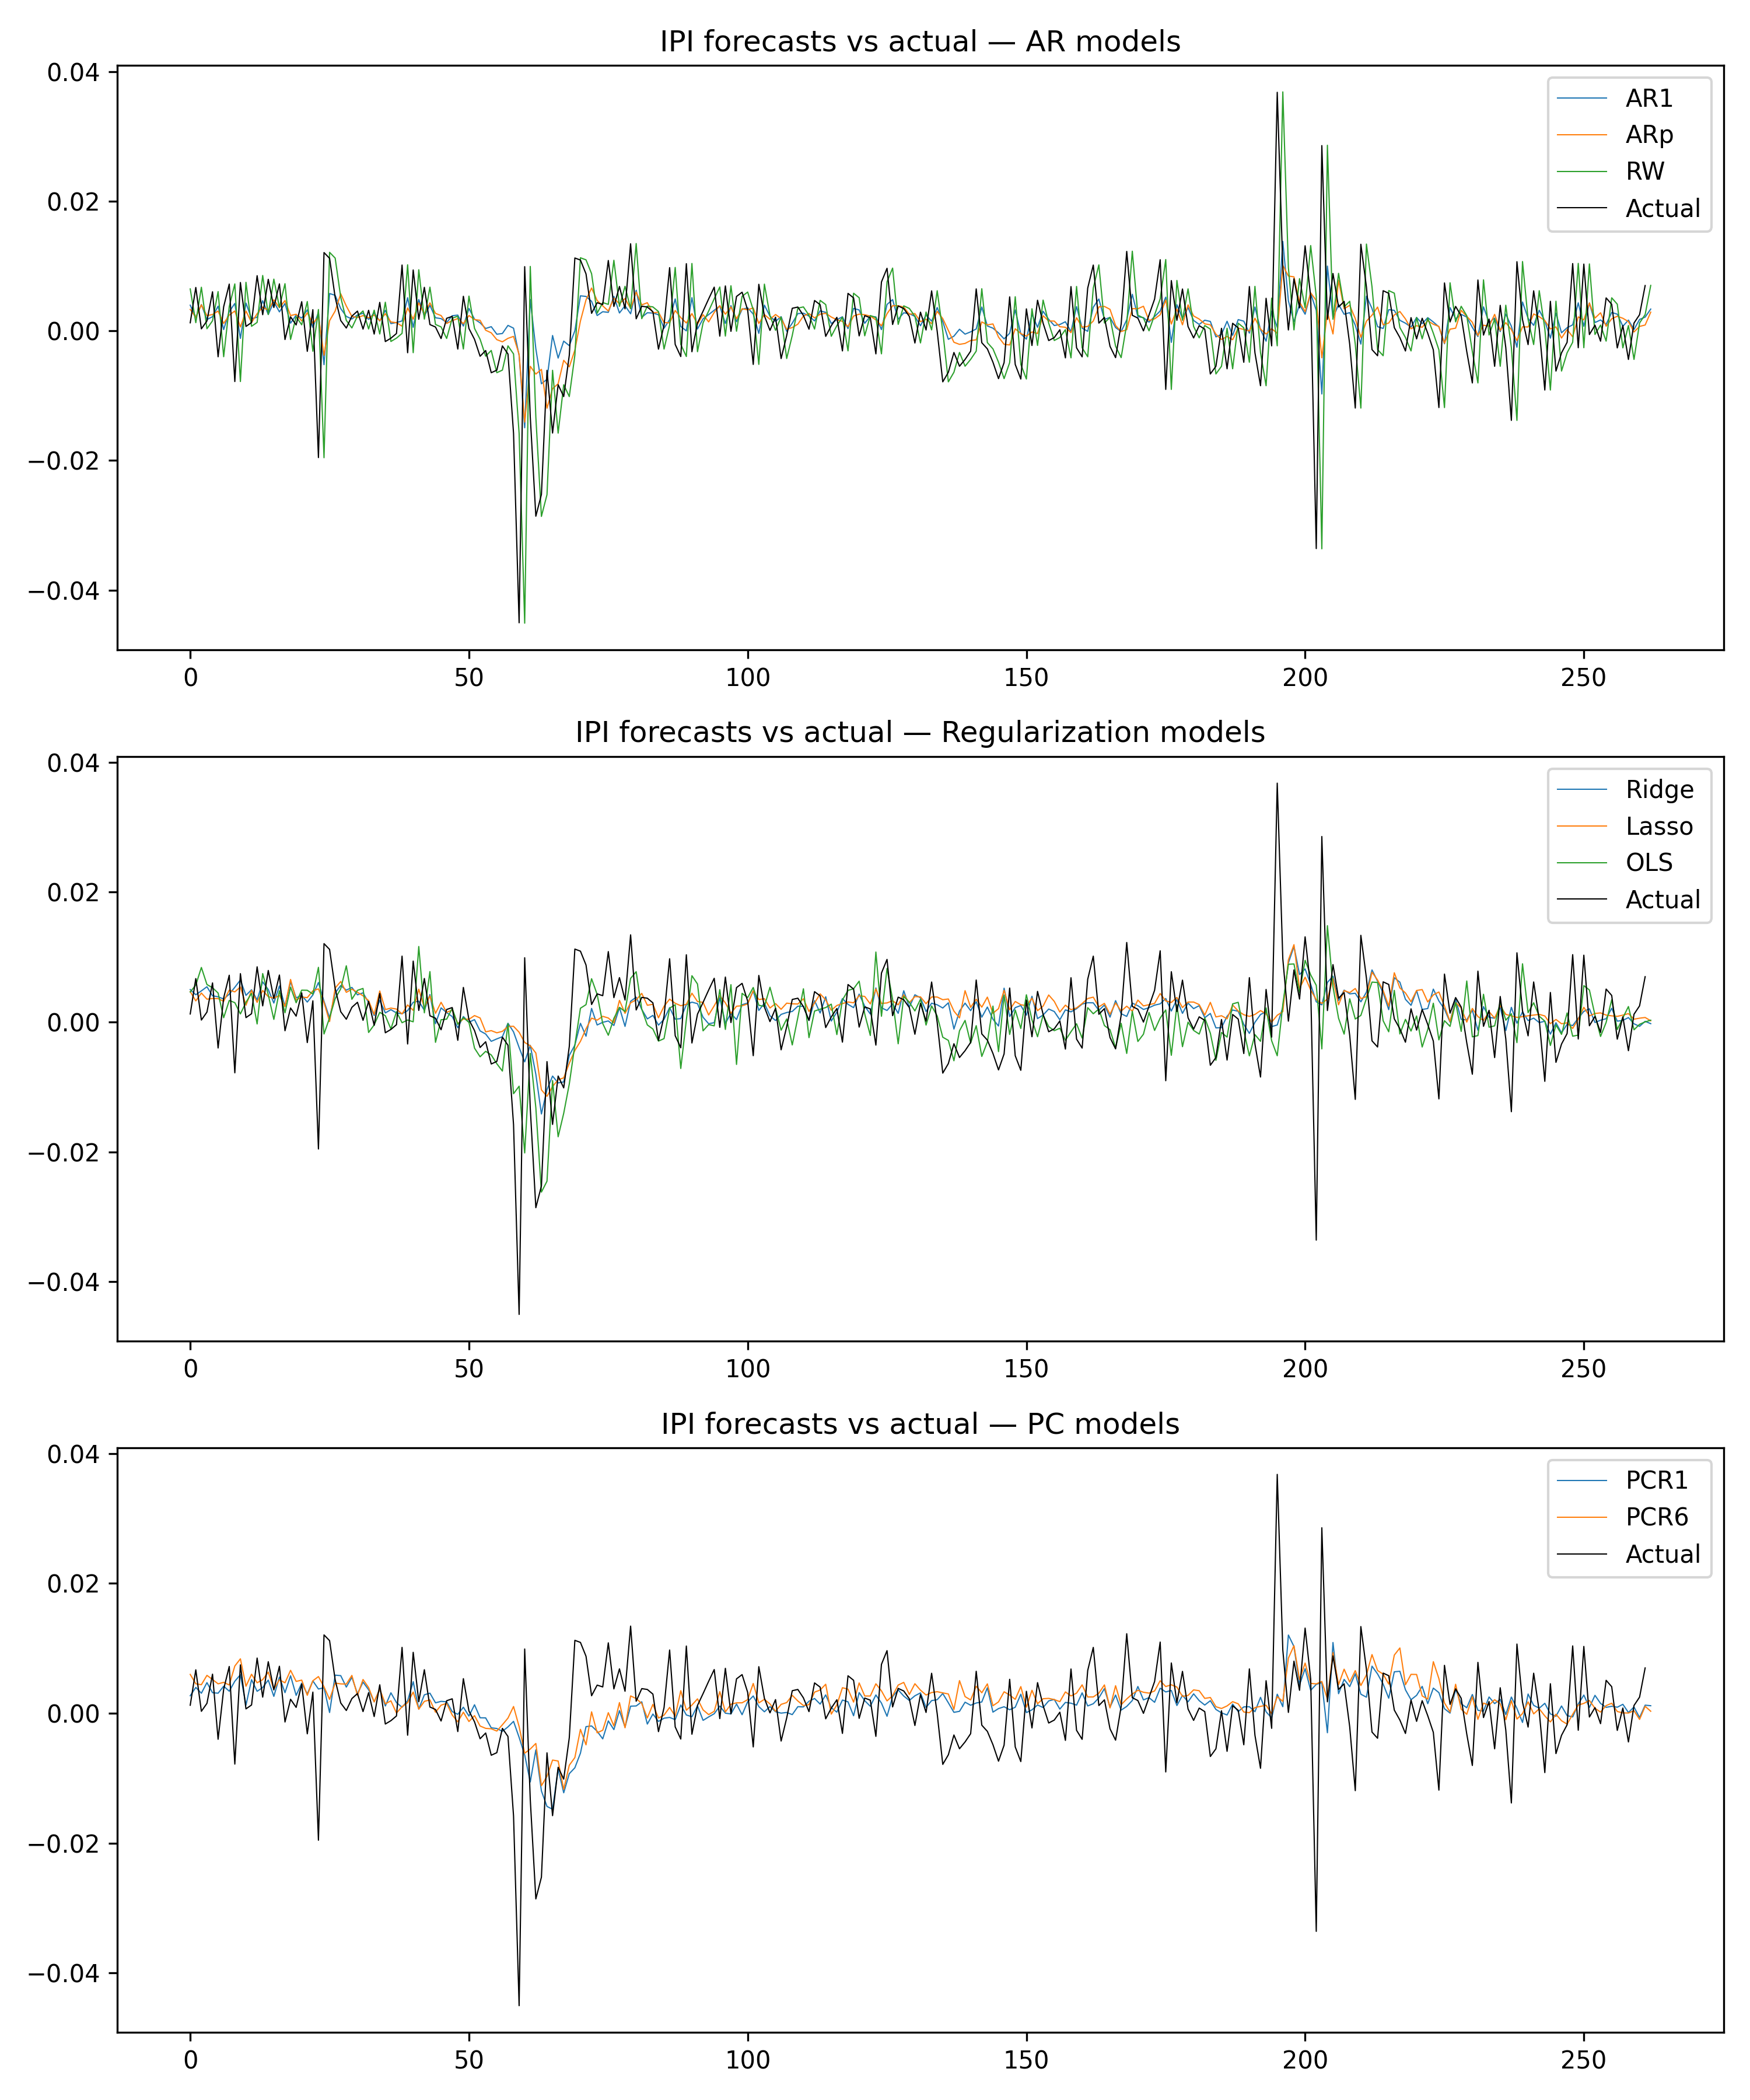
\includegraphics[width=\linewidth]{figures/ipi_forecasts.png}
    \caption{One-step-ahead forecasts vs.\ actual $\Delta\log\,\mathrm{INDPRO}$, by model group.}
    \label{fig:ipi_forecasts}
\end{figure}

\begin{figure}[H]
    \centering
    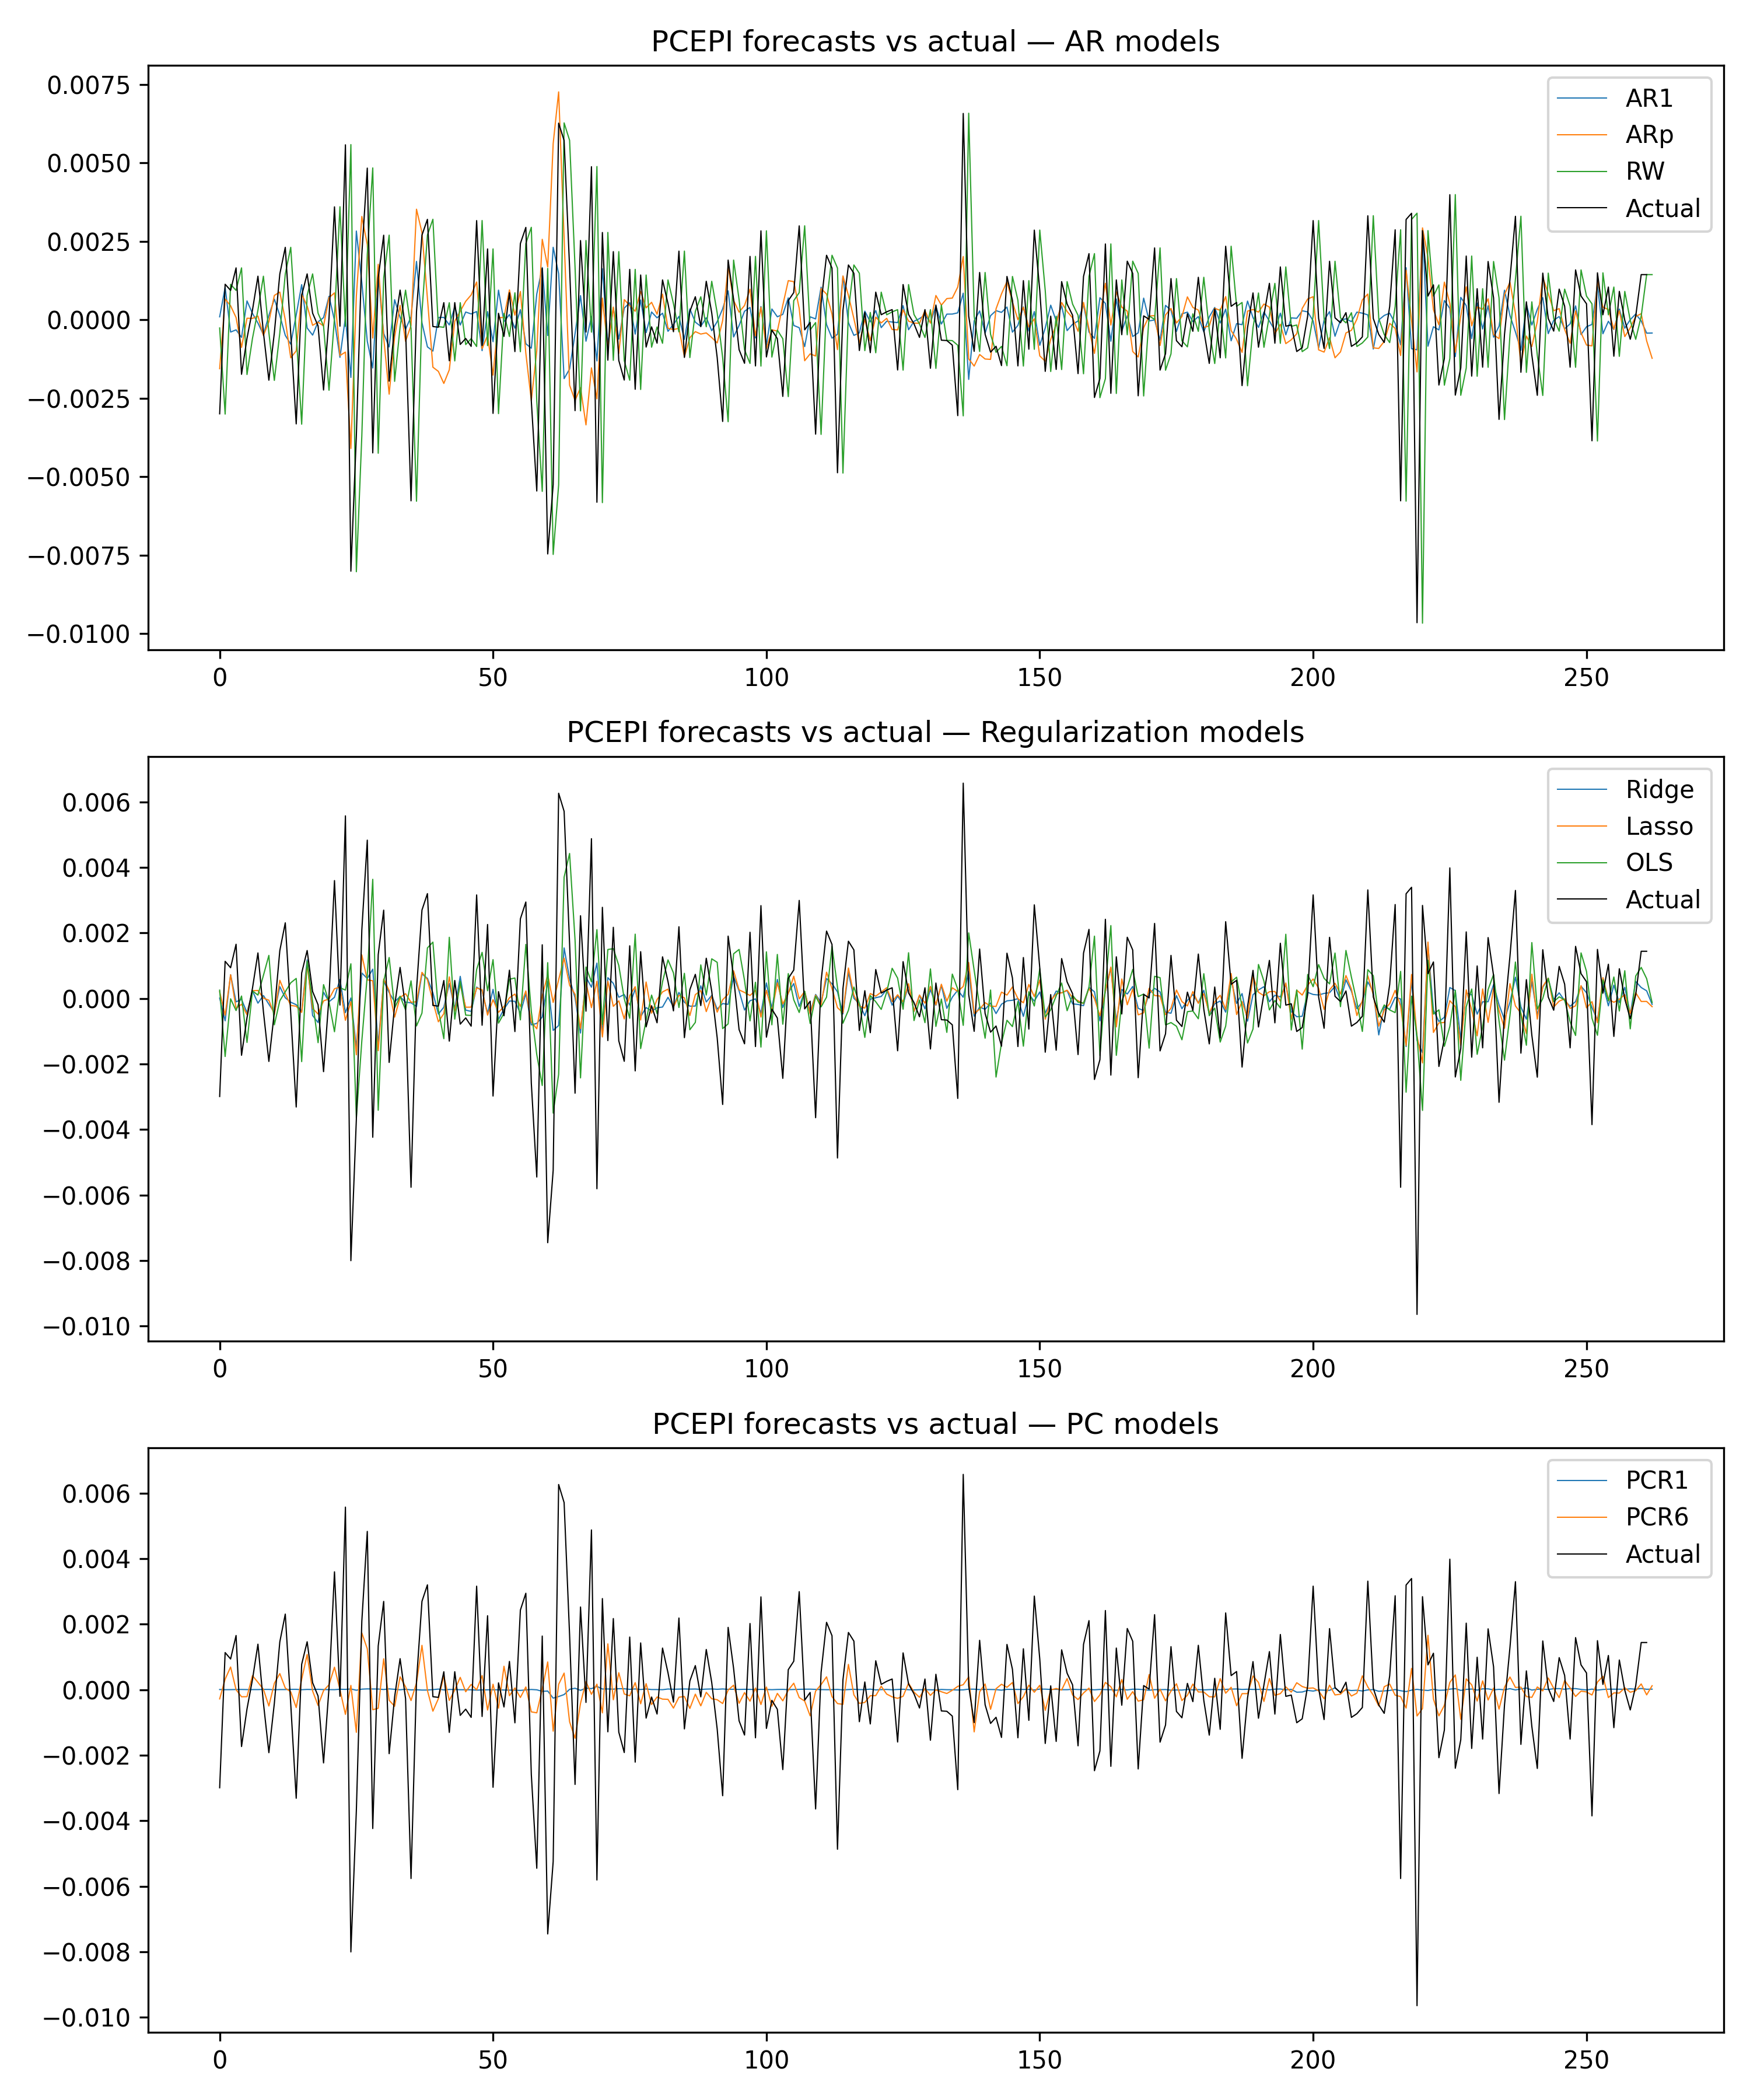
\includegraphics[width=\linewidth]{figures/pcepi_forecasts.png}
    \caption{One-step-ahead forecasts vs.\ actual $\Delta^2\log\,\mathrm{PCEPI}$, by model group. PCR(1) produces nearly flat predictions.}
    \label{fig:pcepi_forecasts}
\end{figure}

Figure~\ref{fig:rescaled} shows the forecasts rescaled to original levels. 
The PCEPI forecasts are surprisingly close to the target variable, which exhibits a relatively smooth trend. This is also evident in the lower scale of the stationary data forecasts.

\begin{figure}[H]
    \centering
    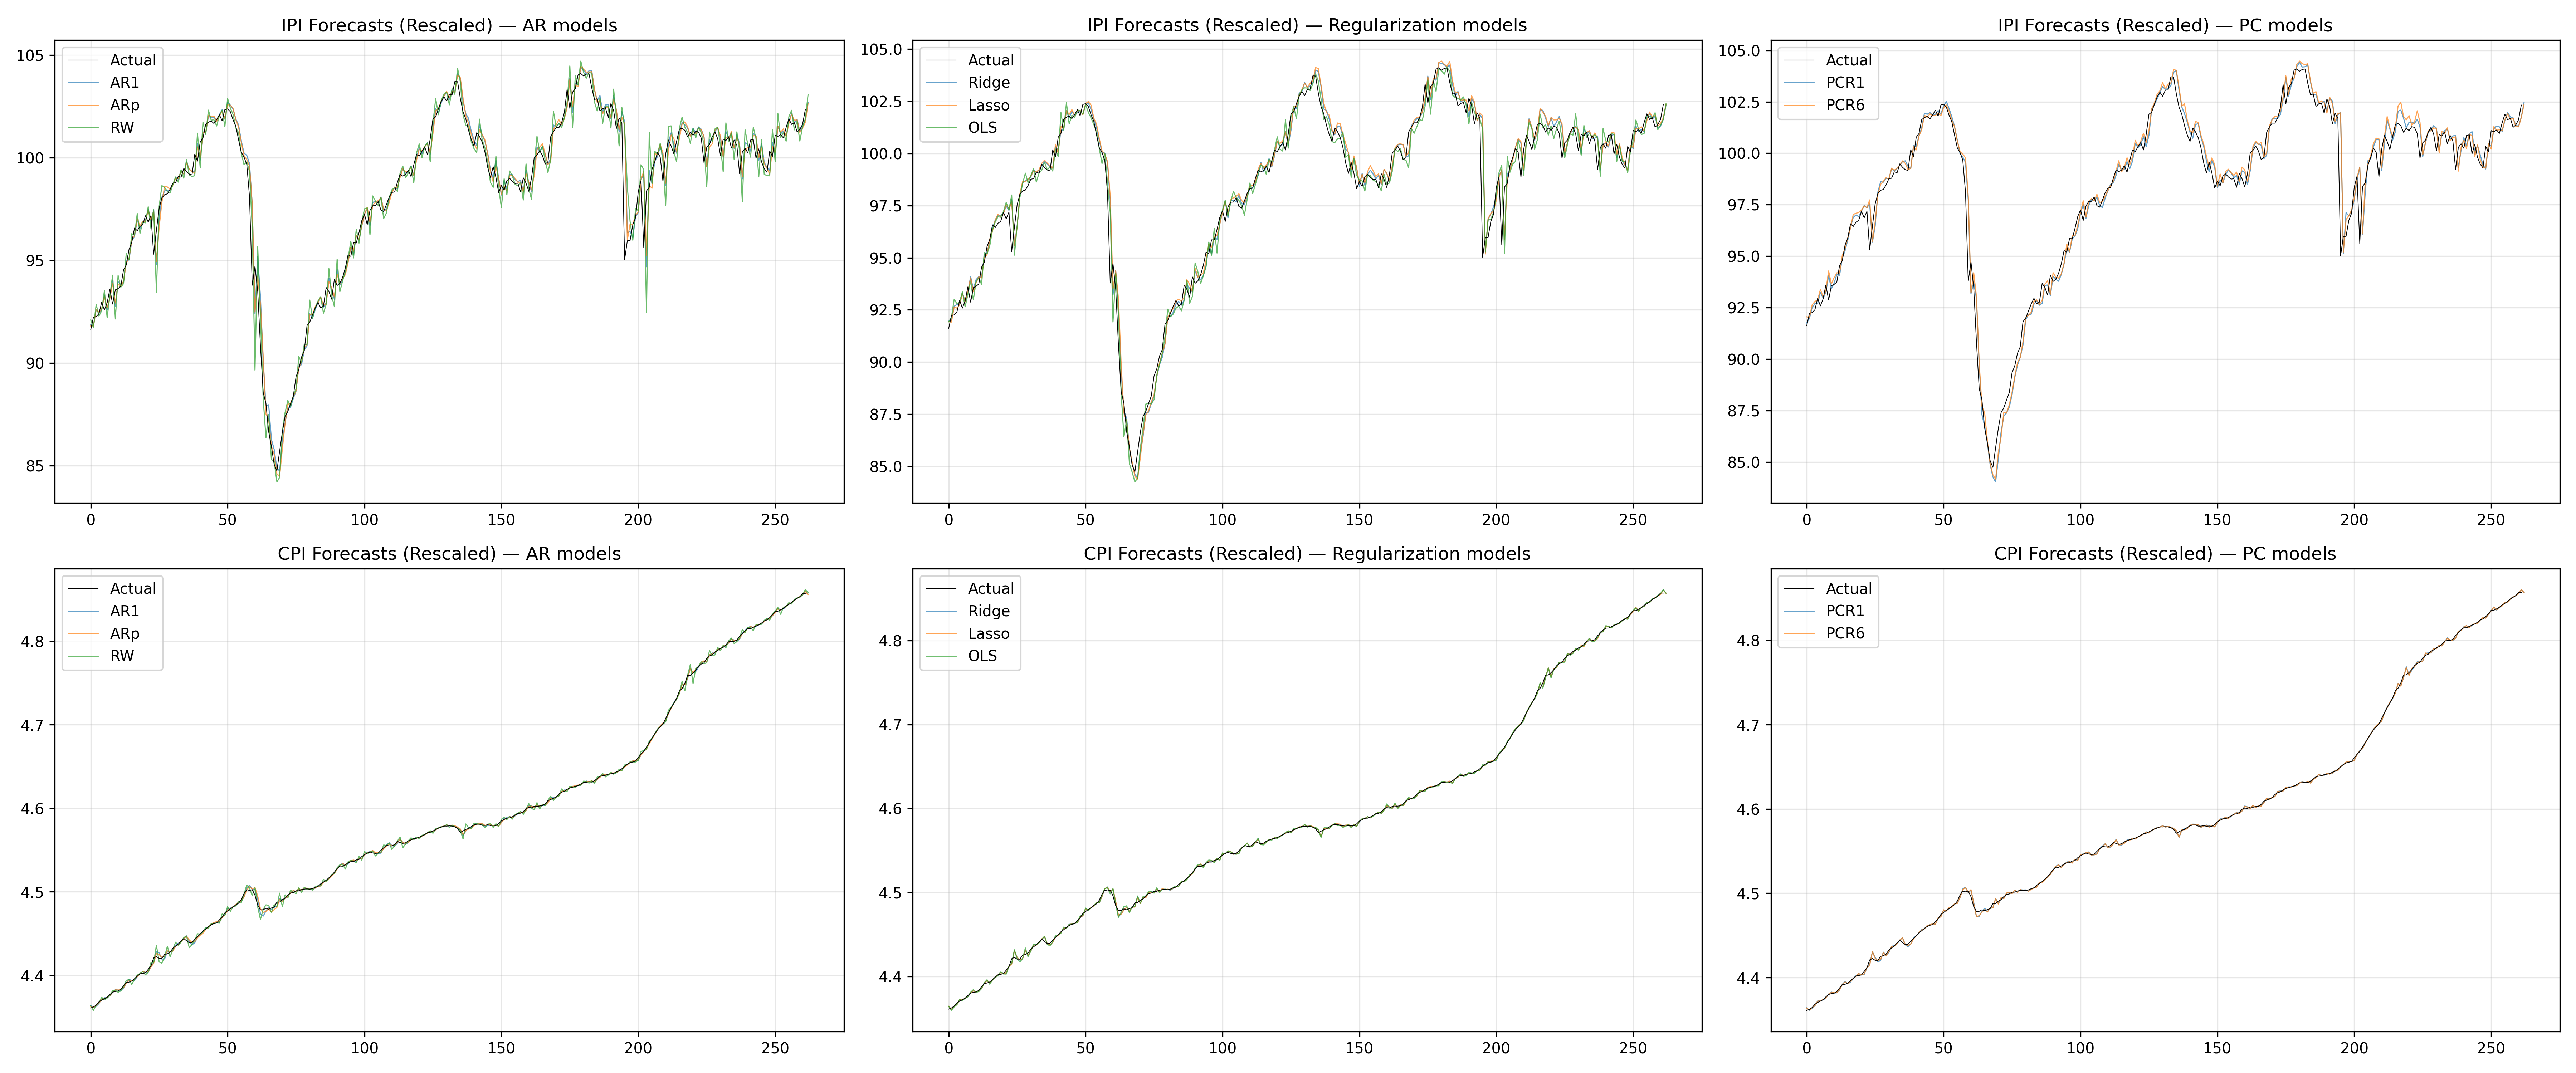
\includegraphics[width=\linewidth]{figures/rescaled_forecasts.png}
    \caption{Forecasts in original levels: INDPRO (top) and $\log\,\mathrm{PCEPI}$ (bottom), by model group.}
    \label{fig:rescaled}
\end{figure}

Figures~\ref{fig:ipi_errors} and \ref{fig:cpi_errors} show the forecast errors over time.
Forecast errors are broadly centred around zero, though with a slight positive bias. The most visible feature is a sharp negative spike around 2008--09, shared by all models,  and positive forecast errors in 2020--2022 for PCEPI, reflecting the unprecedented nature of the COVID-19 shock and its aftermath.
Overall, the simple RW displays visibly larger errors.

\begin{figure}[H]
    \centering
    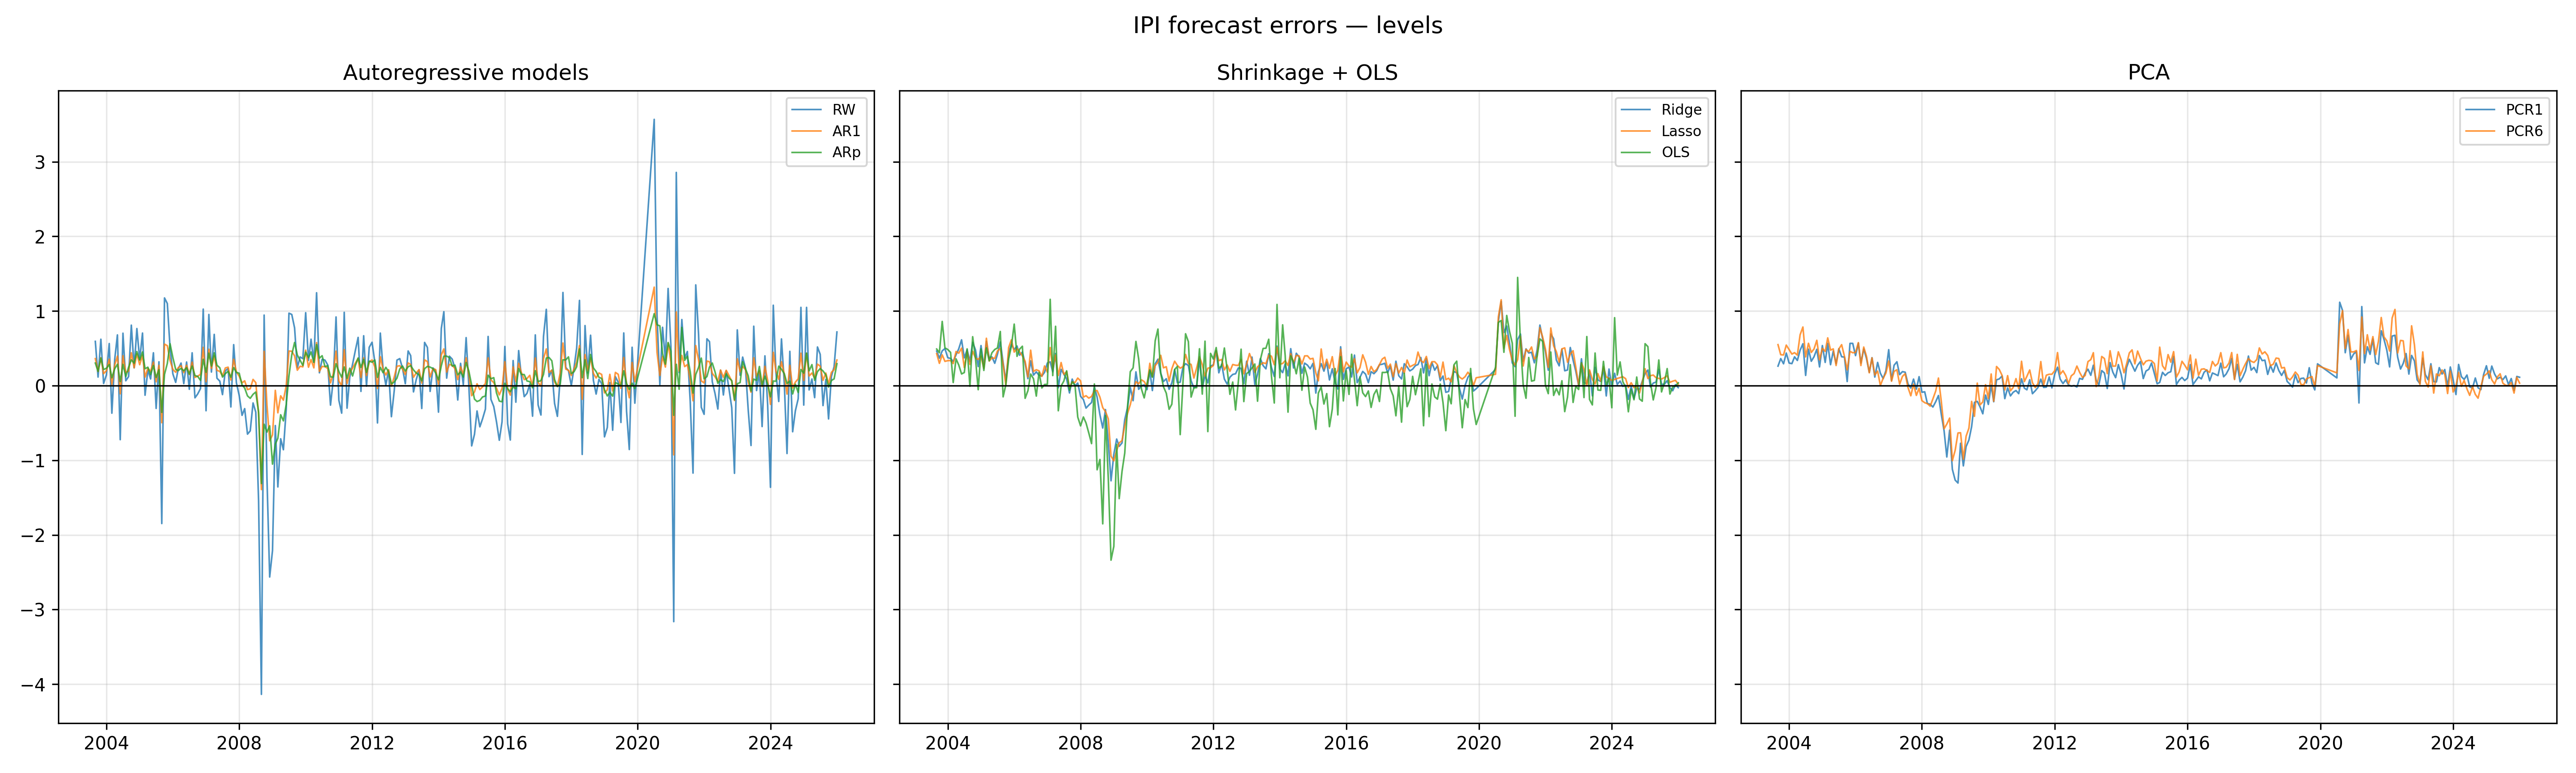
\includegraphics[width=\linewidth]{figures/ipi_forecast_errors.png}
    \caption{Forecast errors for INDPRO levels over the evaluation period, by model group.}
    \label{fig:ipi_errors}
\end{figure}

\begin{figure}[H]
    \centering
    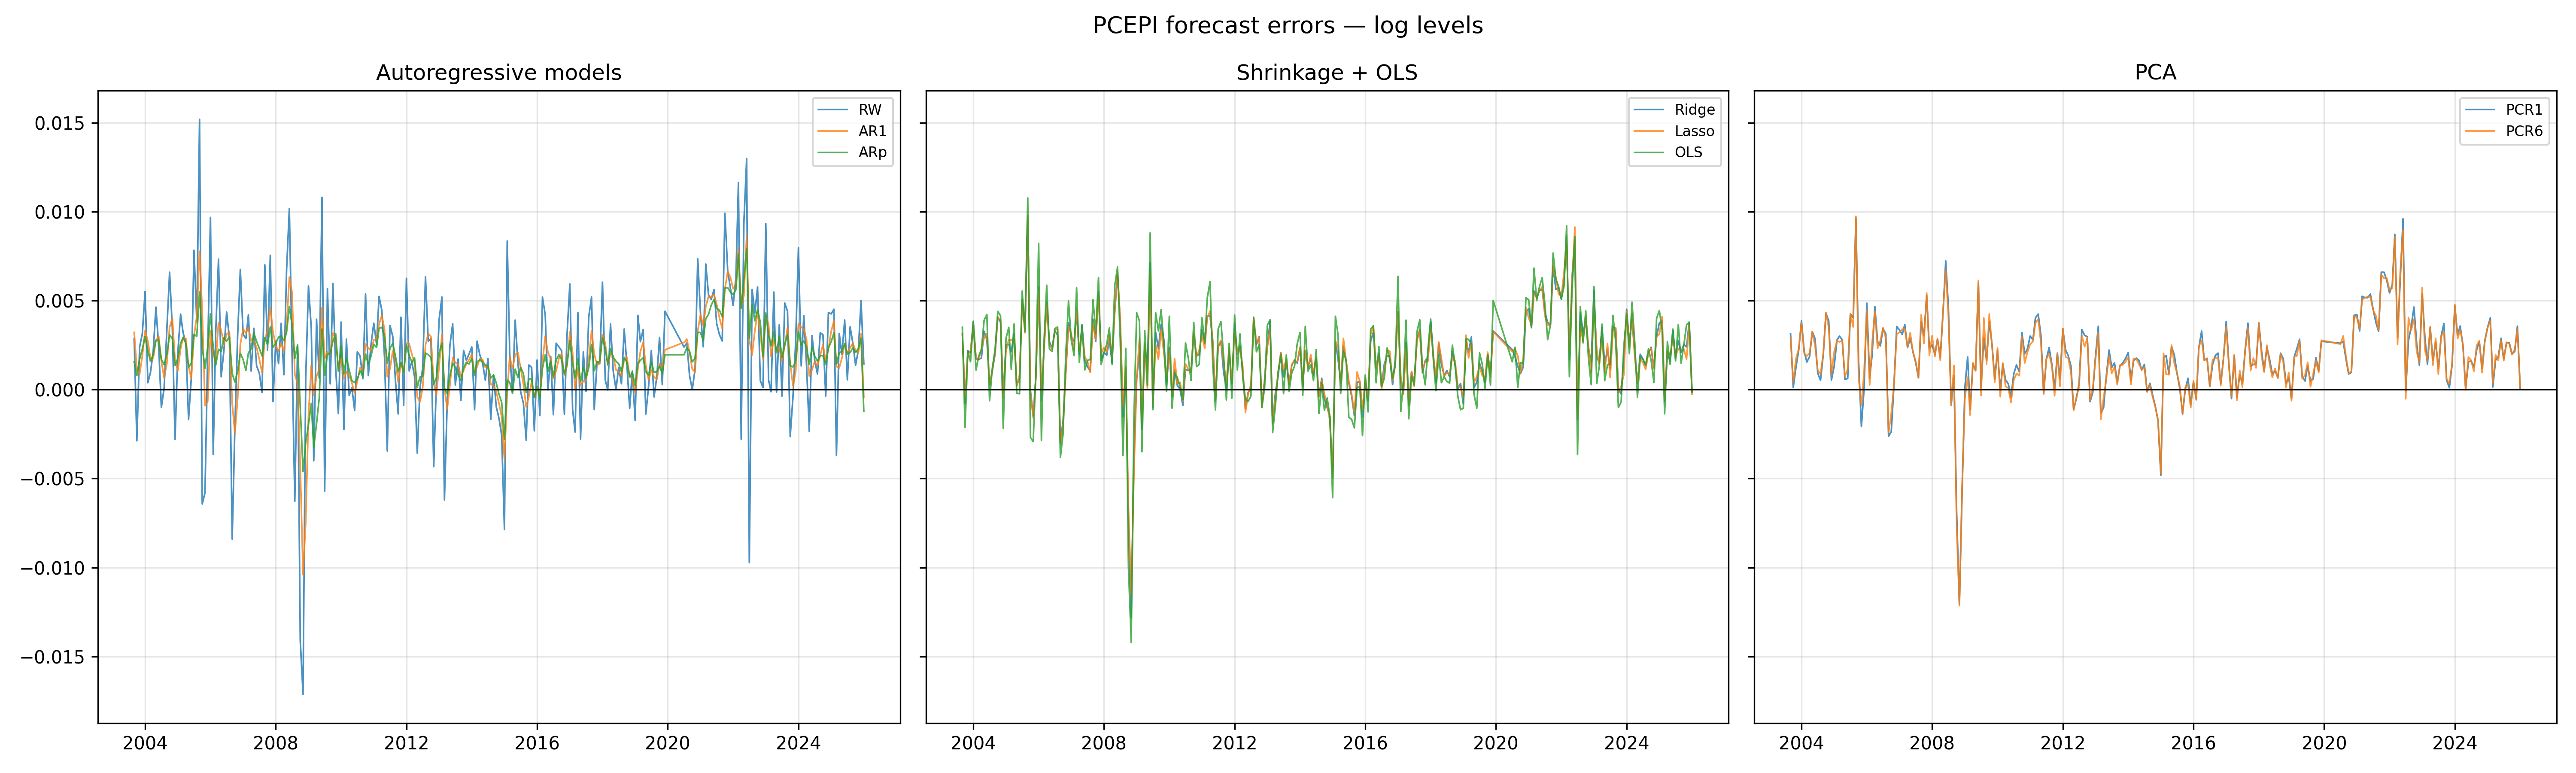
\includegraphics[width=\linewidth]{figures/cpi_forecast_errors.png}
    \caption{Forecast errors for $\log\,\mathrm{PCEPI}$ over the evaluation period, by model group.}
    \label{fig:cpi_errors}
\end{figure}



\subsection{RMSE Comparison and Discussion}
\label{sec:res_rmse}

Tables~\ref{tab:rmse_ipi} and \ref{tab:rmse_cpi} report the RMSE with 95\% HAC confidence intervals to account for
autocorrelation in forecast errors. Differences discussed below are
statistically significant unless otherwise noted.

\begin{table}[H]
    \centering
    \caption{Root Mean Squared Error with 95\% CI --- Industrial Production Index}
    \label{tab:rmse_ipi}
    \begin{tabular}{lrrr}
\toprule
 & RMSE & lower & upper \\
\midrule
ARp & 0.29122 & 0.28801 & 0.29443 \\
AR1 & 0.29841 & 0.29565 & 0.30118 \\
Ridge & 0.32995 & 0.32641 & 0.33350 \\
PCR1 & 0.33677 & 0.33207 & 0.34148 \\
Lasso & 0.33961 & 0.33668 & 0.34255 \\
PCR6 & 0.36538 & 0.36210 & 0.36866 \\
OLS & 0.47146 & 0.46411 & 0.47881 \\
RW & 0.72367 & 0.71308 & 0.73426 \\
\bottomrule
\end{tabular}

\end{table}

\begin{table}[H]
    \centering
    \caption{Root Mean Squared Error with 95\% CI --- PCEPI}
    \label{tab:rmse_cpi}
    \begin{tabular}{lrrr}
\toprule
 & RMSE & lower & upper \\
\midrule
ARp & 0.00245 & 0.00243 & 0.00247 \\
AR1 & 0.00274 & 0.00272 & 0.00277 \\
PCR6 & 0.00287 & 0.00284 & 0.00289 \\
Lasso & 0.00290 & 0.00288 & 0.00293 \\
PCR1 & 0.00292 & 0.00289 & 0.00294 \\
Ridge & 0.00294 & 0.00292 & 0.00297 \\
OLS & 0.00335 & 0.00332 & 0.00337 \\
RW & 0.00421 & 0.00417 & 0.00425 \\
\bottomrule
\end{tabular}

\end{table}

\subsubsection*{Industrial Production}

For both variables, the best model is AR(p), followed by AR(1). 

On the other hand, the worst performer is RW, with a RMSE twice as large as the other autoregressive models. This was expected due to the stationary nature of the variables.
The second-worst model is OLS. This is consistent with the overfitting it typically introduces in high-dimensional settings, and with the effectiveness of shrinkage introduced by Ridge and Lasso in improving out-of-sample performance.
Shrinkage and dimensionality-reduction models perform better than OLS and worse than AR models, with RMSEs that are statistically indistinguishable from each other.

The best multivariate model for INDPRO is Ridge, performing slightly better than Lasso and PCR(1). This might indicate that a larger panel is more appropriate for forecasting industrial production, as highlighted by a higher number of non-zero coefficients selected by Lasso.
PCR(1) performs better than PCR(6), which might be due to the correlation of the first component to real activity.
For PCEPI, shrinkage and PCR models perform similarly, and are not statistically different.

These findings suggest that shrinkage and dimensionality reduction effectively offset the curse of dimensionality. However, for the target variables under analysis, using a large panel of predictors does not substantially improve over the AR(p) benchmarks.

% ══════════════════════════════════════════════════════════════════════════════
\section{Conclusion}
\label{sec:conclusion and Limitations}

This paper applied the forecasting framework of De Mol, Giannone and Reichlin (2008) to the FRED-MD panel, comparing eight models for one-step-ahead prediction of industrial production and inflation in an expanding-window evaluation.
While shrinkage and principal component regression outperform OLS -- with similar performance -- they do not beat the AR(p) models for inflation and industrial production forecasts.

Two limitations are worth noting. First, hyperparameters are fixed on the first training window rather than re-tuned recursively, which may not reflect true real-time conditions.
Second, an expanding window is used rather than a rolling window -- this dilutes the relevance of more recent data, which might be more informative especially after regime shifts. 

\section{References}

\begin{thebibliography}{99}
    \bibitem{demol2008}
    De Mol, C., Giannone, D., \& Reichlin, L. (2008).
    Forecasting using a large number of predictors: Is Bayesian shrinkage a valid alternative to principal components?
    \textit{Journal of Econometrics}, 146(2), 318--328.

    \bibitem{mccracken2016}
    McCracken, M. W., \& Ng, S. (2016).
    FRED-MD: A monthly database for macroeconomic research.
    \textit{Journal of Business \& Economic Statistics}, 34(4), 574--589.
\end{thebibliography}

 \end{document}